%% Template for a preprint Letter or Article for submission
%% to the journal Nature.
%% Written by Peter Czoschke, 26 February 2004
%%

\documentclass[12pt]{article}

%% make sure you have the nature.cls and naturemag.bst files where
%% LaTeX can find them

\usepackage{scicite,graphicx,rotating}
\usepackage{times}


\title{Supplementary Material: 
``Climate change decouples drought from early winegrape harvests in France''}

%% Notice placement of commas and superscripts and use of &
%% in the author list
%/Users/bcook/Desktop/WINELIZZIE/MANUSCRIPT/figures_eps_png/SUPP_fig_12_JJA_clim_regplots.png

\author{Benjamin I Cook$^{1,2}$ \& Elizabeth M Wolkovich$^{3,4}$}


\begin{document}

\maketitle

\section*{Regional GHD Analyses}
\noindent To analyze each site individually, we regressed the GHD for each site in GHD-Core against CRU climate data averaged within one degree of the site location. As with GHD-Core, temperature is the dominant control on GHD in all eight regional series (Supplementary Figures 4--11), and all the temperature regressions are highly significant ($p\le0.01$). For the period 1901--1980, the temperature sensitivities (regression slopes) across sites range from a minimum of $-3.70$ days \textsuperscript{o}C\textsuperscript{--1} at SRv to $-7.39$ days \textsuperscript{o}C\textsuperscript{--1} at Cha1. Significant ($p\le0.05$) moisture sensitivities (precipitation and PDSI) are also found at seven of the eight sites: Als, Bor, Bur, Cha1, Lan, LLV, and Swi. At the eighth site, SRv, the precipitation regression is marginally significant ($p=0.055$) and is insignificant for PDSI.\\
\indent At all sites, GHD temperature sensitivities remain significant for the 1981--2007 interval, indicating that temperature remains an important control on winegrape phenology in more recent decades. By contrast, most sites show a significant weakening of the two moisture sensitivities. Both the precipitation and PDSI regressions with GHD become insignificant ($p>0.05$) during 1981--2007 for Bor, Bur, Cha1, Lan, LLV, and Swi. At SRv, only precipitation was marginally significant for 1901--1980, and this regression weakens considerably. At Als, the PDSI regression becomes insignificant, while precipitation does not change appreciably. Analyses of the individual regional GHD series therefore support the general conclusions drawn from analyses of the GHD-Core composite index, demonstrating an overall large-scale weakening of moisture controls on GHD in Western Europe.

\section*{Temperature versus Moisture Comparisons}
\noindent We hypothesize that, in Western Europe, moisture impacts on winegrape phenology occur primarily through the indirect effect of moisture on growing season temperatures. Further, we argue that because of anthropogenic warming trends in recent decades, winegrape phenology has become decoupled from moisture variability. Here we, present evidence in support of these hypotheses.\\
\indent A strong connection between soil moisture and warm season temperatures over the Mediterranean and Western Europe has been well established \cite{Fischer2007,Miralles2014}, occurring primarily through the control of soil moisture on surface energy partitioning. In regions where evapotranspiration is limited by the supply of moisture at the surface, wetter soils will lead to increases in evapotranspiration and latent heat flux at the expense of sensible heating, keeping surface soil and air temperatures relatively cool. Conversely, if soils are dry, sensible heat fluxes will dominate, and soil and air temperatures will be higher. If these are the primary physics operating in our GHD-Core region, we would therefore expect negative relationships between temperature and precipitation or PDSI.\\
\indent Indeed, for both MJJ (Supplementary Figure 12) and JJA (Supplementary Figure 14) we can see significant negative relationships between both temperature and precipitation and PDSI during the 1901--1980 interval. The relationships are generally stronger during JJA, when solar energy inputs are larger and land-atmosphere interactions are expected to be stronger. During the more recent interval (1981--2007), the temperature moisture relationships generally weaken, especially during JJA. Additionally, temperature during 1981--2007 are substantially warmer compared to 1901--1980, reflecting recent warming trends driven primarily by anthropogenic greenhouse gas forcing. This additional warmth (unrelated to moisture variability), combined with the apparent weakening of the temperature-moisture coupling strength itself, all support our conclusions regarding the mechanisms by which moisture influences GHD variability and the recent weakening of this relationship.

\section*{Monte-Carlo Analyses}
\noindent Interpretations of the composite climate anomaly analyses (Figure 4, main manuscript) and comparisons of climate distributions (Supplemental Figure 15, top panel) for extreme early harvest years may be affected by sampling uncertainties or biases, especially during the post 1981 period when the number of early harvest years to sample from is small. For example, from 1600--1981, 72 years qualify as early harvests with GHD-Core anomalies of -7.7 days or earlier. Because of the last years represented in the climate reconstructions, however, from 1981 to 2007 only 18 years qualify for PDSI, 13 years for temperature, and 11 years for precipitation. To estimate the impact on our analyses of these potential sampling uncertainties, we conducted a Monte-Carlo analysis where, in each of 10,000 iterations, we resampled climate anomalies from the early harvest years with replacement. For both intervals (1600--1980 and 1981--2007) and each iteration, we resampled $n$ times, where $n$ is equal to the number of early harvest years from 1981--2007 (so 11 for precipitation, 13 for temperature, and 18 for PDSI).\\
\indent Kernal density functions for the 10,000 resampled mean precipitation and PDSI anomalies are shown in the bottom panels of Supplemental Figure 15. As in the main analysis, PDSI shows the strongest shift with early harvest dates before and after 1980. The 1\textsuperscript{st} and 99\textsuperscript{th} percentiles of the resampled mean distributions are non-overlapping for the two periods (1600--1980$=-0.053$; 1981--2007$=0.094$). Additionally, repeating the One Sided Student's t-test and Wilcoxon Ranksum test found 97\% and 93\% of the iterations significant at a $p<=0.05$, implying that sampling uncertainties are unlikely to be large enough to affect our interpretations of the differences in PDSI during early harvest years. For precipitation, as before, repeating the tests for all the iterations yields.

\bibliographystyle{naturemag}
\bibliography{/Users/bcook/Dropbox/LATEX/mylib.bib}   % name your BibTeX data base

%% TABLE: MEAN DATES
\begin{sidewaystable}
%\begin{table}
\small
\caption{\small Regional GHD series from DAUX used in construction of the GHD-Core composite series. Included are the three letter codes for each site, their geographic locations (units of decimal degrees), and their mean harvest dates (day of year) for various intervals.}
\centering
\begin{tabular}{| l l | r r | c c c c c p{5cm} |}
\hline
 \bf GHD Series & \bf Site Code & \bf Lat & \bf Lon & \bf 1600-1900 & \bf 1600-1980 & \bf 1901-1950 & \bf 1951-1980 & \bf 1981-2007 \\
\hline
Alsace	& Als & 48.17 & 7.28 & 282.81 & 281.87 & 272.12 & 287.16	 & 277.70 \\
Bordeaux	& Bor	& 45.18 & -0.75	& 269.01 & 	268.22	&  263.85 &  270.41 &  259.75\\
Burgundy	& Bur	& 47.32	& 5.04	& 269.92	& 270.07	& 269.44	& 272.58	& 262.15\\
Champagne 1	& Cha1	& 47.98	& 4.28	& 266.88	& 267.52	& 267.01	& 270.02	& 264.92\\
Langeudoc & Lan	& 43.60 & 3.87	& 272.43 &	270.28	& 260.97	& 266.88	& 263.40\\
Low Loire Valley	& LLV	& 47.15	& 0.22	& 286.12	& 284.61	& 282.69	& 282.56	& 275.33\\
Southern Rhone Valley	& SRv	& 43.98	& 5.05	& 269.20	& 269.10	& 268.84	& 268.46	& 257.87\\
Switzerland (Lake Geneva)	& Swi	& 46.57	& 6.52	& 286.39	& 283.87	& 273.86	& 275.22	& 263.00\\
\hline
\end{tabular}
\end{sidewaystable}

%% TABLE: SERIAL COMPLETION
% FINAL CHECK: DONE
\begin{table}
\small
\caption{\small For each regional GHD series used in GHD-Core, the fraction of years with observations for various time intervals.}
\centering
\begin{tabular}{l c c c c c}
\hline
 & \bf 1354-2007 & \bf 1600-1900 & \bf 1600-2007 & \bf 1800-2007 & \bf 1900-2007\\
\hline
Als	& 0.401 & 0.578 & 0.642 & 0.837	 & 0.824\\
Bor	 & 0.500 & 0.648 & 0.738 & 0.995 & 0.991\\
Bur & 	0.925	& 0.997	& 0.990	& 0.986	& 0.972\\
Cha1	& 0.280	& 0.259	& 0.449	& 0.880	& 0.981\\
Lan	& 0.442 & 0.635	& 0.689	& 0.438	& 0.833\\
LLV	& 0.310	& 0.332	& 0.498	& 0.976	& 0.963\\
SRv	& 0.690	& 0.970	& 0.951	& 0.942	& 0.898\\
Swi 	& 0.749	& 1.00 & 1.00	& 1.00	& 1.00\\
\hline
\end{tabular}
\end{table}
%\end{sidewaystable}

%% TABLE: CROSS SITE CORRELATIONS
% FINAL CHECK: DONE
\begin{table}
\small
\caption{\small Spearman's rank correlations (1354-2007) between the various regional GHD series used to construct GHD-Core. GHD series were NOT detrended prior to the correlation analysis.}
\centering
\begin{tabular}{c c c c c c c c c}
\hline
& Als & Bor & Bur & Cha1 & Lan & LLV & SRv & Swi \\
\hline
Als &1.00 &  &  &  &  &  &  & \\
Bor & 0.601 & 1.00 &  &  &  &  &  & \\
Bur & 0.574 & 0.615 & 1.00 &  &  &  &  & \\
Cha1 & 0.632 & 0.675 & 0.799 & 1.00 &  &  &  & \\
Lan & 0.550 & 0.467 & 0.450 & 0.655 & 1.00 &  &  & \\
LLV & 0.503 & 0.712 & 0.776 & 0.709 & 0.359 & 1.00 &  & \\
SRv & 0.414 & 0.249 & 0.456 & 0.346 & 0.765 & 0.456 & 1.00 & \\
Swi & 0.604 & 0.554 & 0.562 & 0.569 & 0.705 & 0.697 & 0.501 & 1.00\\
%Als &1.00 & 0.601 & 0.574 & 0.632 & 0.550 & 0.503 & 0.414 & 0.604\\
%Bor & 0.601 & 1.00 & 0.615 & 0.675 & 0.467 & 0.712 & 0.249 & 0.554\\
%Bur & 0.574 & 0.615 & 1.00 & 0.799 & 0.450 & 0.776 & 0.456 & 0.562\\
%Cha1 & 0.632 & 0.675 & 0.799 & 1.00 & 0.655 & 0.709 & 0.346 & 0.569\\
%Lan & 0.550 & 0.467 & 0.450 & 0.655 & 1.00 & 0.359 & 0.765 & 0.705\\
%LLV & 0.503 & 0.712 & 0.776 & 0.709 & 0.359 & 1.00 & 0.456 & 0.697\\
%SRv & 0.414 & 0.249 & 0.456 & 0.346 & 0.765 & 0.456 & 1.00 & 0.501\\
%Swi & 0.604 & 0.554 & 0.562 & 0.569 & 0.705 & 0.697 & 0.501 & 1.00\\
\hline
\end{tabular}
%\end{sidewaystable}
\end{table}

%% TABLE: GHD ANOMALIES
% FINAL CHECK: DONE
\begin{table}
\small
\caption{\small Day of year anomalies in the regional GHD series used to construct GHD-Core. Anomalies are calculated relative to the baseline mean dates from 1600-1900. Also included are results for the GHD-Core index and GHD-All, composited from all 27 regional GHD series in DAUX. For GHD-Core and GHD-All, the harvest date anomalies were calculated for the regional series individually before averaging together. Because the regional GHD series are not all equally represented in all years, anomalies in GHD-Core and GHD-All are slightly non-zero for the baseline averaging period (1600--1900).}
\centering
\begin{tabular}{l c c c c c}
\hline
& \bf 1600-1900 & \bf 1600-1980 & \bf 1901-1950 & \bf 1951-1980 & \bf 1981-2007\\
\hline
Als	& 0	& -0.94 & -10.69 & 4.35 & -5.11\\
Bor	& 0 & -0.79 & -5.16 & 1.40 & -9.26\\
Bur	& 0	& 0.15	& -0.48	& 2.66	& -7.78\\
Cha1	& 0	& 0.64	& 0.13	& 3.14	& -1.96\\
Lan & 0 & -2.14 & -11.46 & -5.55 & -9.03\\
LLV	& 0	& -1.51	& -3.42	& -3.56	& -10.79\\
SRv & 0	& -0.10	& -0.36	& -0.74	& -11.33\\
Swi	& 0	& -2.52	& -12.53	& -11.17	& -23.39\\
\hline
GHD-Core & -0.32 & -1.02	& -5.16 & -1.11 & -10.24\\
GHD-All	& -0.25 & -0.85 & -5.13 & 0.36 & -8.91\\
\hline
\end{tabular}
%\end{sidewaystable}
\end{table}

%% TABLE: GHD STANDARD DEVIATIONS
% FINAL CHECK: DONE
\begin{table}
\small
\caption{\small As Table 4, but for inter-annual standard deviation.}
\centering
\begin{tabular}{l c c c c c}
\hline
& \bf 1600-1900 & \bf 1600-1980 & \bf 1901-1950 & \bf 1951-1980 & \bf 1981-2007\\
\hline
Als	& 8.74	& 9.56	& 9.12	& 7.09	& 8.74\\
Bor	& 9.51	& 9.00	& 6.27	& 7.00	& 9.56\\
Bur	& 9.61 & 9.19 & 6.55 & 8.11 & 7.97\\
Cha1 & 8.81 & 8.88 & 7.85 & 10.12 & 8.64\\
Lan & 8.63 & 9.03 & 6.51 & 5.69 & 5.39\\
LLV	& 10.29 & 9.21 & 6.56 & 8.01 & 7.41\\
SRv & 8.68 & 8.46 & 8.62 & 5.55 & 5.93\\
Swi	& 10.09	& 10.71	& 7.19	& 6.68	& 8.11\\
\hline
GHD-Core & 7.67 & 7.49 & 5.39 & 6.24 & 7.10\\
GHD-All	& 7.03 & 7.02 & 5.55 & 6.55 & 6.75\\
\hline
\end{tabular}
%\end{sidewaystable}
\end{table}

\begin{sidewaystable}[ht]
\centering
\caption{Coefficients and p-values from ordered logit models of wine quality data (on a scale of 0 to 5) and grape harvest dates (GHD) and CRU May-July seasonal temperatures for the periods 1900-1980 and 1981-2001. For more details on data and analyses see the Methods section in the main text.} 
\begin{tabular}{||r||l|l||l|l||}
  \hline
 & GHD: 1900-1980 & GHD: 1981-2001 & Temp: 1900-1980 & Temp: 1981-2001 \\ 
  \hline
Red Bordeaux & -0.117 ($<$0.01) & -0.133 (0.03) & 1.244 ($<$0.01) & 1.308 (0.01) \\ 
  White Bordeaux & -0.084 ($<$0.01) & -0.079 (0.14) & 0.951 ($<$0.01) & 1.109 (0.02) \\ 
  Red Burgundy & -0.102 ($<$0.01) & -0.101 (0.18) & 0.403 (0.06) & 0.612 (0.23) \\ 
  White Burgundy & -0.093 (0.02) & -0.144 (0.07) & 0.564 (0.04) & 1.262 (0.03) \\ 
   \hline
\end{tabular}
\end{sidewaystable}% latex table generated in R 3.1.2 by xtable 1.7-4 package
% Sun Apr 19 19:38:06 2015

\begin{sidewaystable}[ht]
\centering
\caption{Coefficients and p-values from  ordered logit models of wine quality data (on a scale of 0 to 5) and CRU May-July seasonal precipitation and Palmer Drought Severity Index (PDSI) for the periods 1900-1980 and 1981-2001. For more details on data and analyses see the Methods section in the main text.} 
\begin{tabular}{||r||l|l||l|l||}
  \hline
 & Prec: 1900-1980 & Prec: 1981-2001 & PDSI: 1900-1980 & PDSI: 1981-2001 \\ 
  \hline
Red Bordeaux & -0.013 ($<$0.01) & -0.011 (0.12) & -0.457 ($<$0.01) & -0.119 (0.61) \\ 
  White Bordeaux & -0.014 ($<$0.01) & -0.014 (0.06) & -0.291 (0.02) & -0.234 (0.32) \\ 
  Red Burgundy & -0.018 ($<$0.01) & 0 (0.96) & -0.273 (0.03) & 0.12 (0.64) \\ 
  White Burgundy & -0.011 (0.05) & -0.013 (0.08) & -0.101 (0.52) & -0.199 (0.41) \\ 
   \hline
\end{tabular}
\end{sidewaystable}

\pagebreak

%% THESE COMMANDS ARE USED TO RESET THE SUPPLEMENTAL FIGURE NAMES
\renewcommand{\figurename}{Supplementary Figure}
\setcounter{figure}{0}
%\renewcommand{\thefigure}{}

\begin{figure}
\center
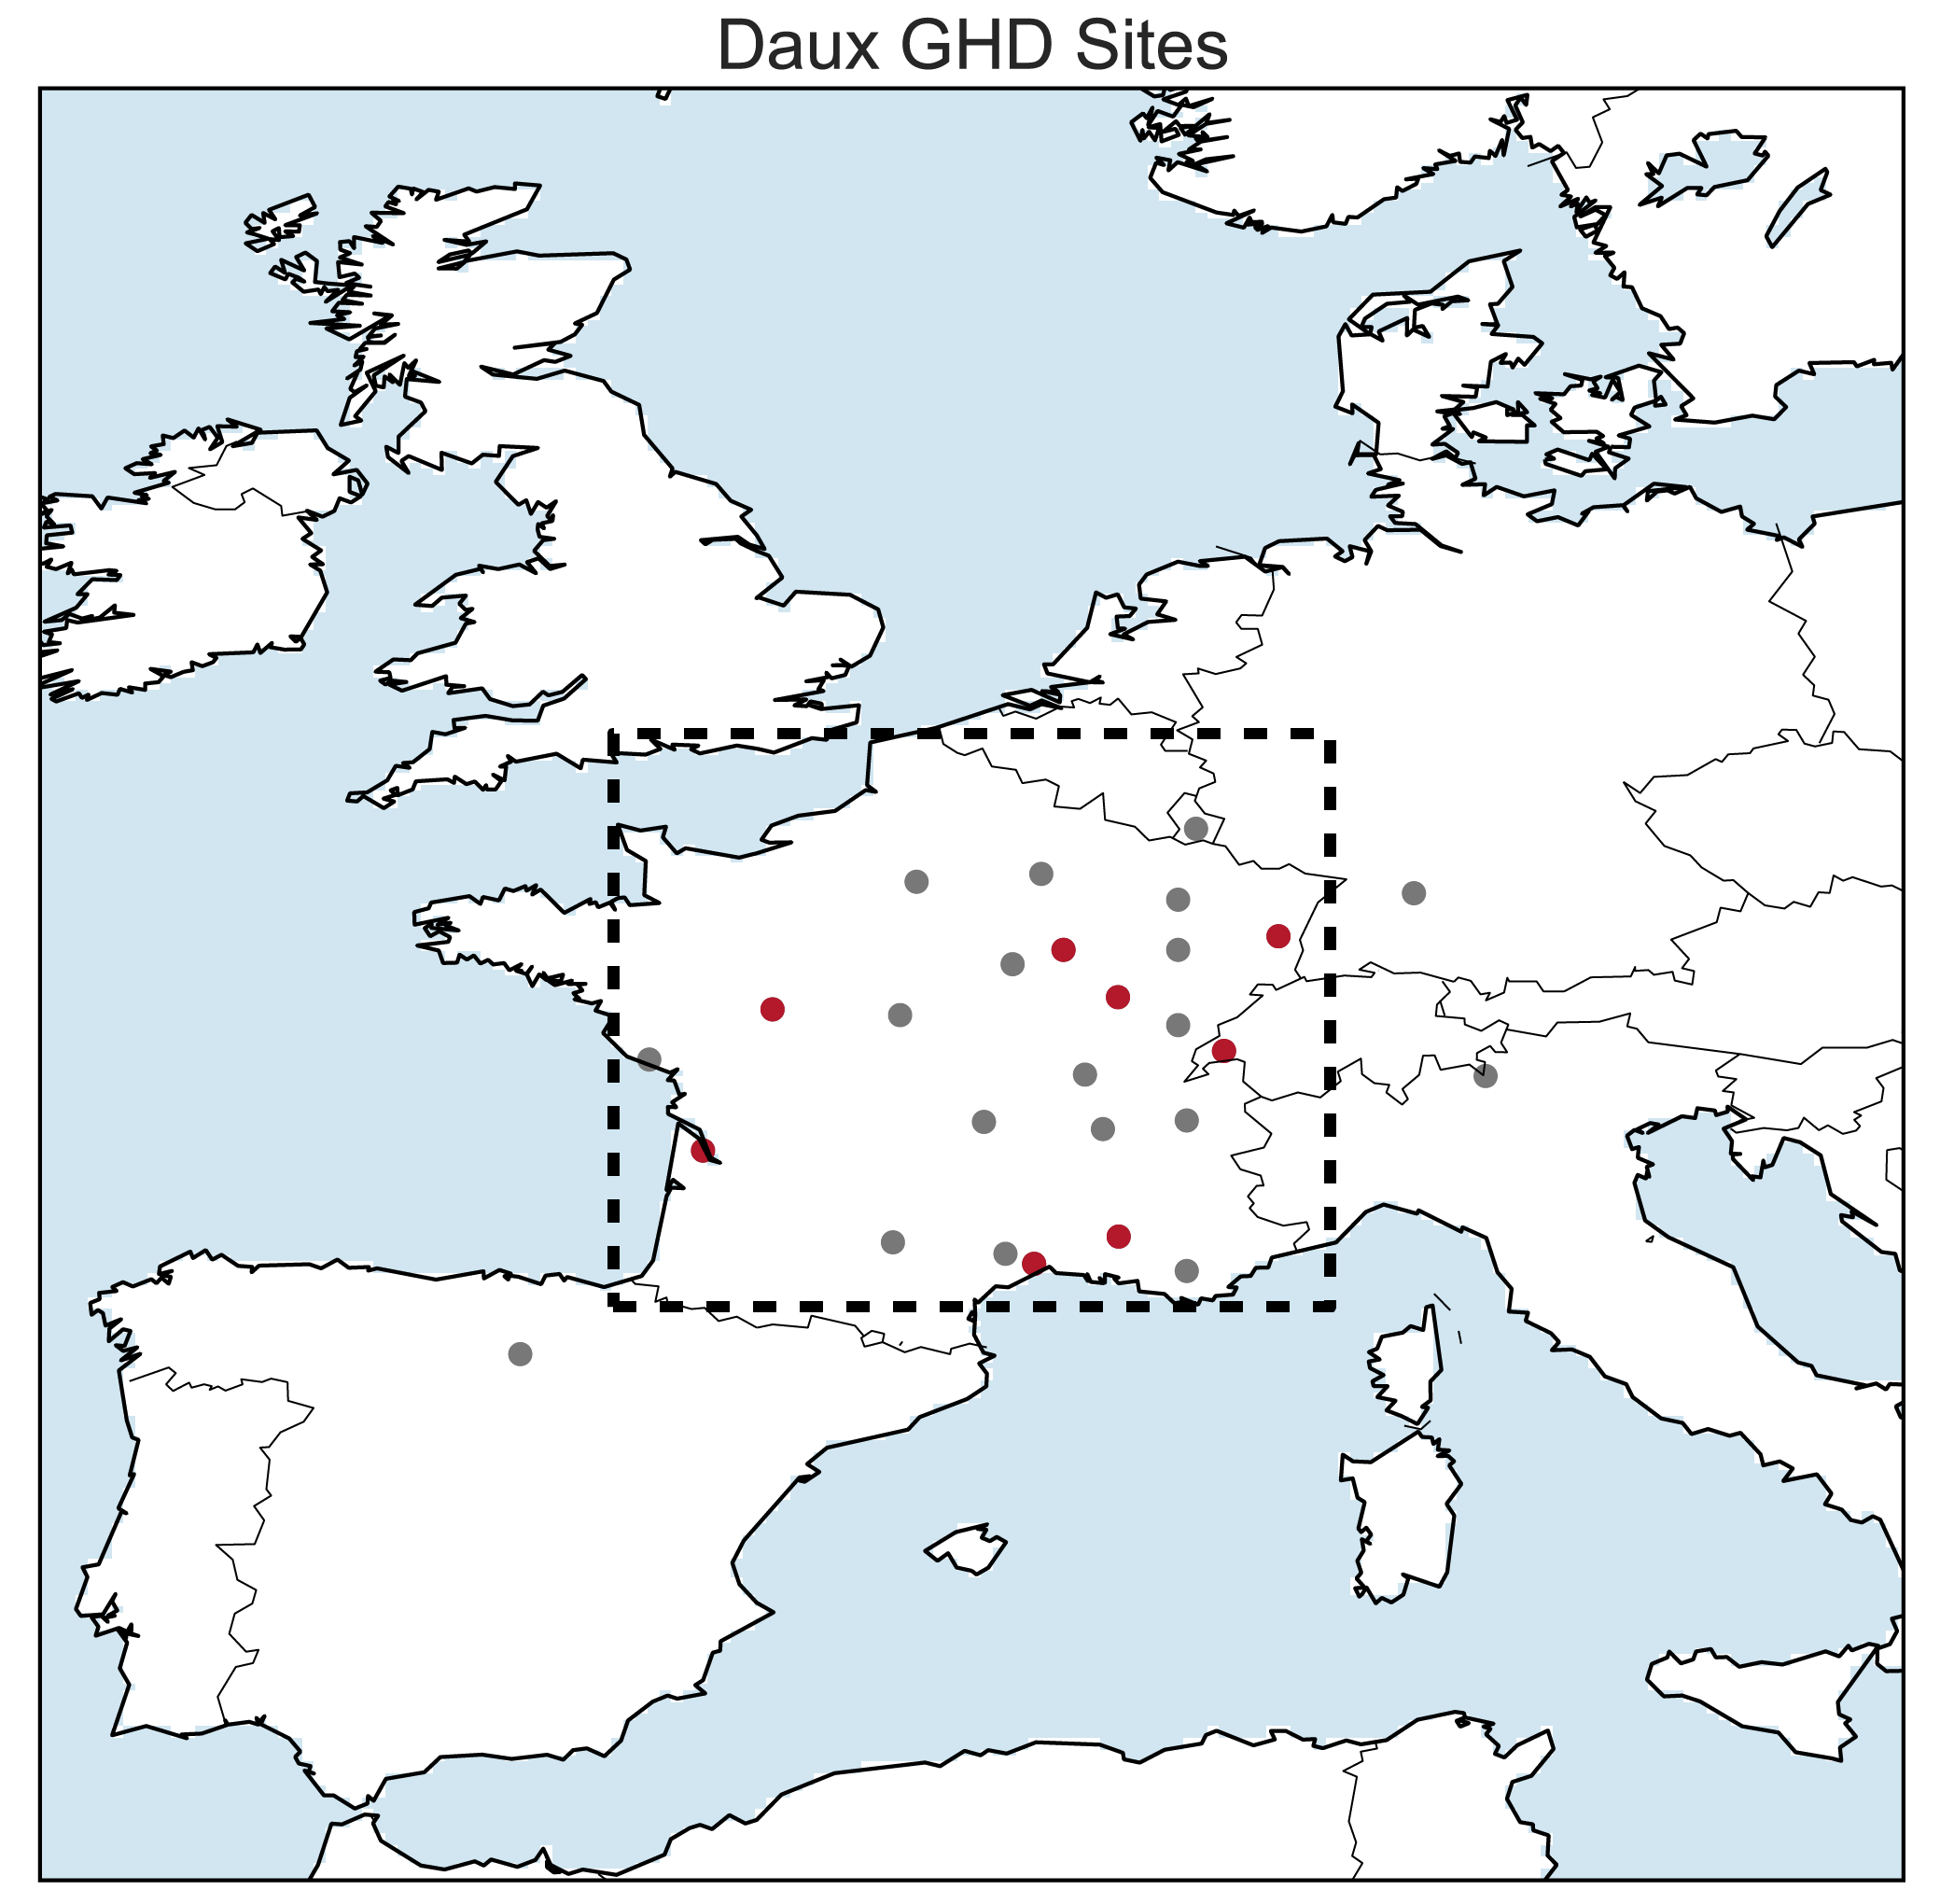
\includegraphics[width=1.0\columnwidth,scale=2]{SUPP_fig_01_map_sites.png}
\caption{Geographic locations for all 27 regional GHD time series in DAUX. Highlighted in red are the sites that comprise the GHD-Core index: Alsace (Als), Bordeaux (Bor), Burgundy (Bur), Champagne 1 (Cha1), Languedoc (Lan), the Lower Loire Valley (LLV), the Southern Rhone Valley (SRv), and Switzerland at Lake Geneva (Swi). The dashed black box indicates the GHD-Core region (2\textsuperscript{o}W--8\textsuperscript{o}E, 43\textsuperscript{o}N--51\textsuperscript{o}N) over which climate anomalies from the CRU instrumental climate datasets and the three climate reconstructions were averaged for the various regression analyses.}
\end{figure}

\begin{figure}
\center
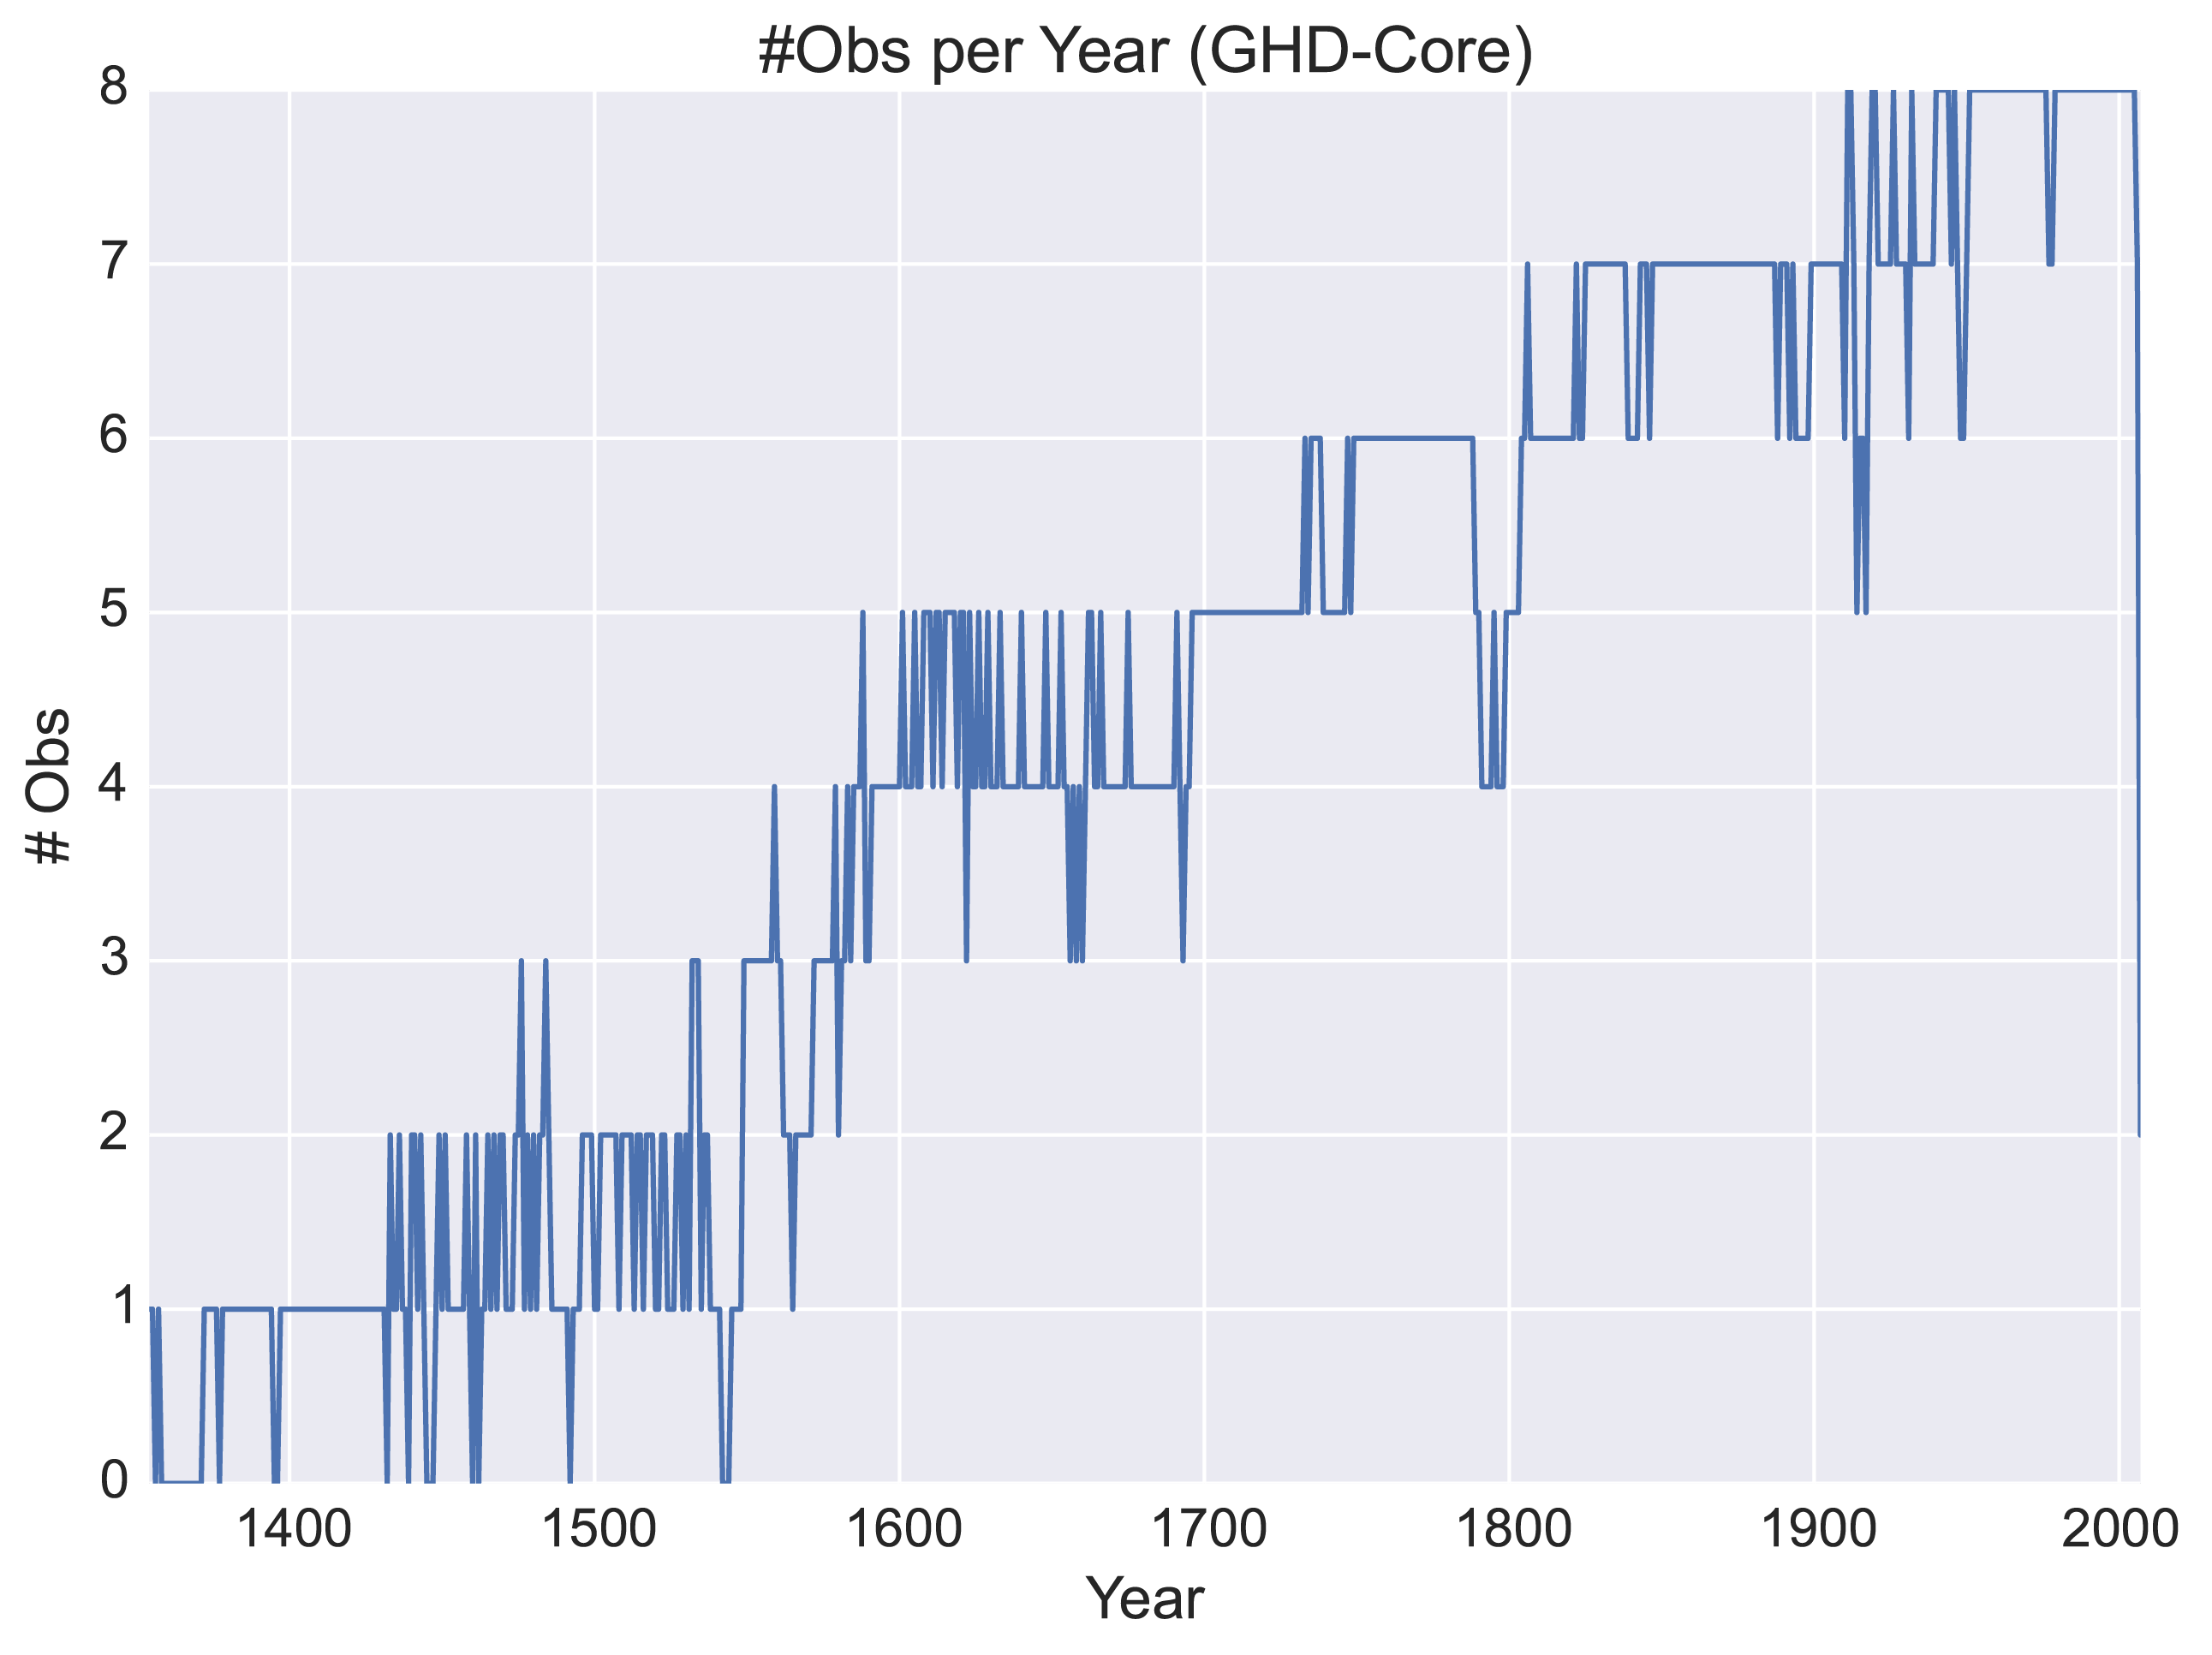
\includegraphics[width=1.0\columnwidth,scale=2]{SUPP_fig_02_numobs.png}
\caption{Number of observations (i.e., regional GHD series) represented in each year of the GHD-Core index.}
\end{figure}

\begin{sidewaysfigure}
\center
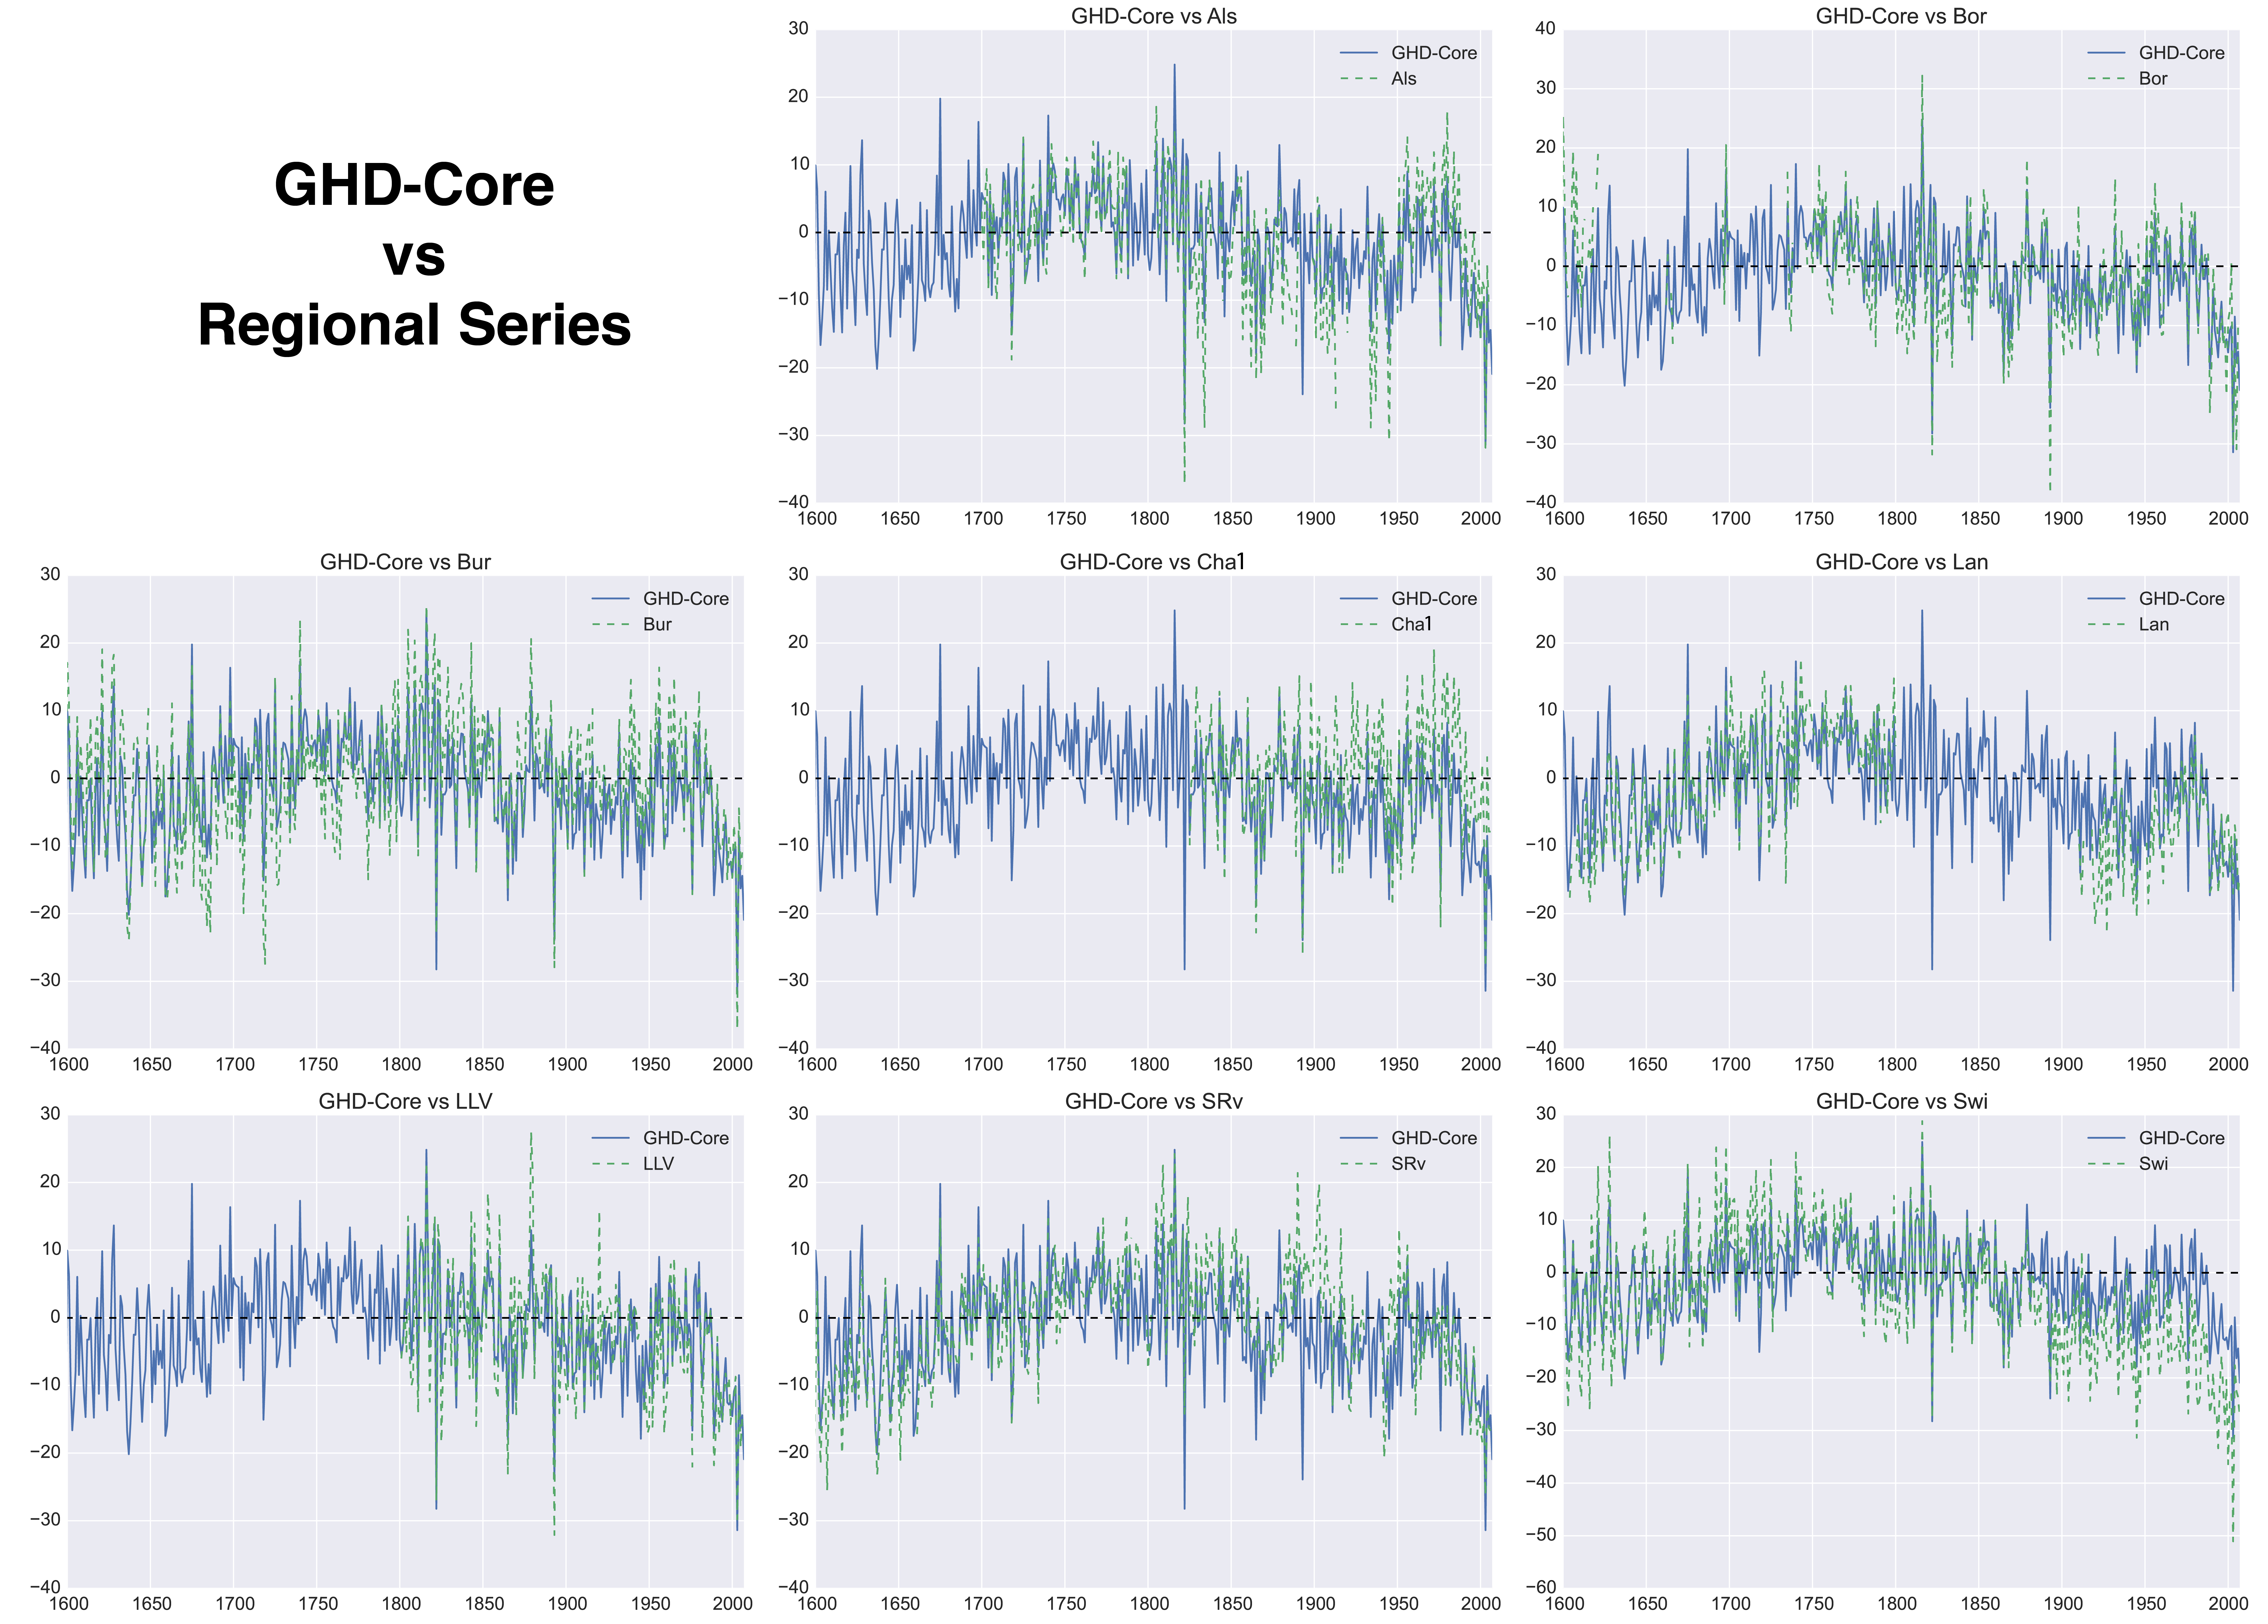
\includegraphics[width=1.0\columnwidth,scale=2]{SUPP_fig_03_core_vs_sites.png}
\caption{Time series (1600--2007) of GHD-Core (blue sold line) and each individual regional GHD series (green dashed lines) used in the construction of GHD-Core.}
\end{sidewaysfigure}

\begin{figure}
\center
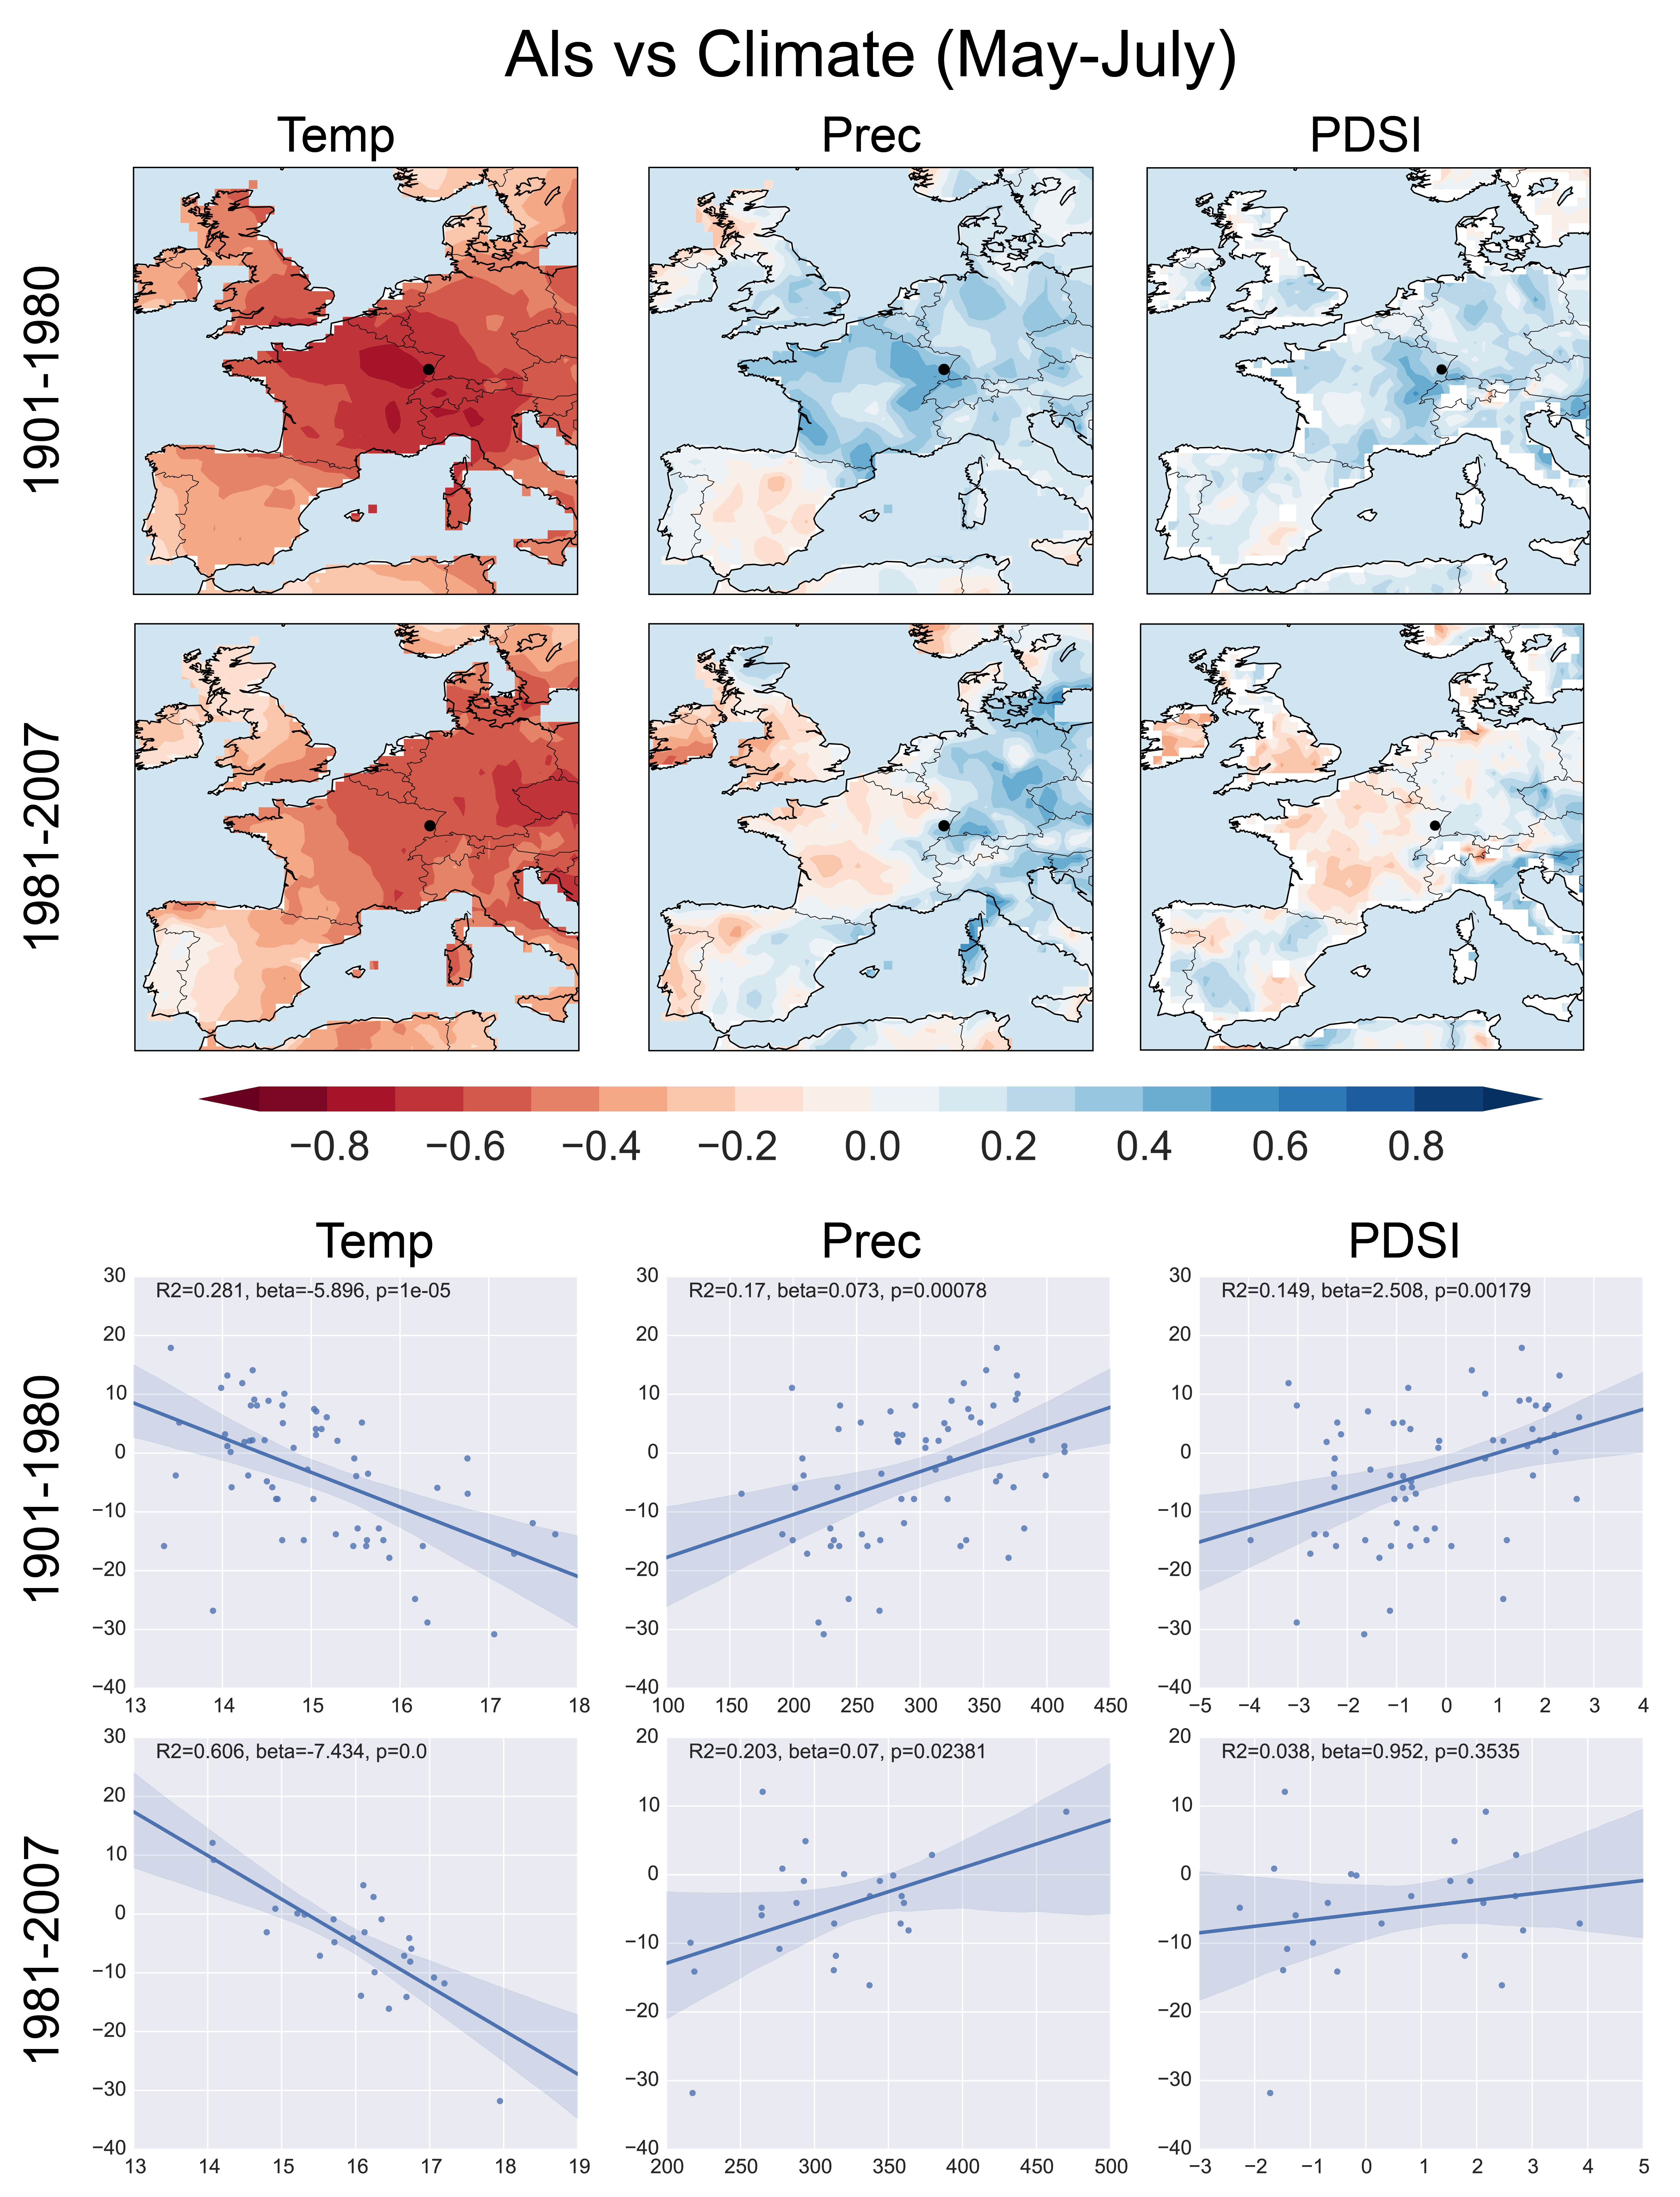
\includegraphics[width=.9\columnwidth,scale=2]{SUPP_fig_04_Als_MJJ_climate_onedeg.png}
\caption{Comparisons between the GHD series from ALS and May-June-July temperature, precipitation, and PDSI from the CRU 3.21 climate grids. Top panels: point-by-point Spearman's rank correlations for 1901--1980 and 1981--2007 (location of ALS is shown by the black dot). Bottom panels: linear regression plots for the same intervals against CRU climate data averaged within one degree of the site location. For the correlation maps, both the climate time series and GHD series were linearly detrended; the regression analyses were not.}
\end{figure}

\begin{figure}
\center
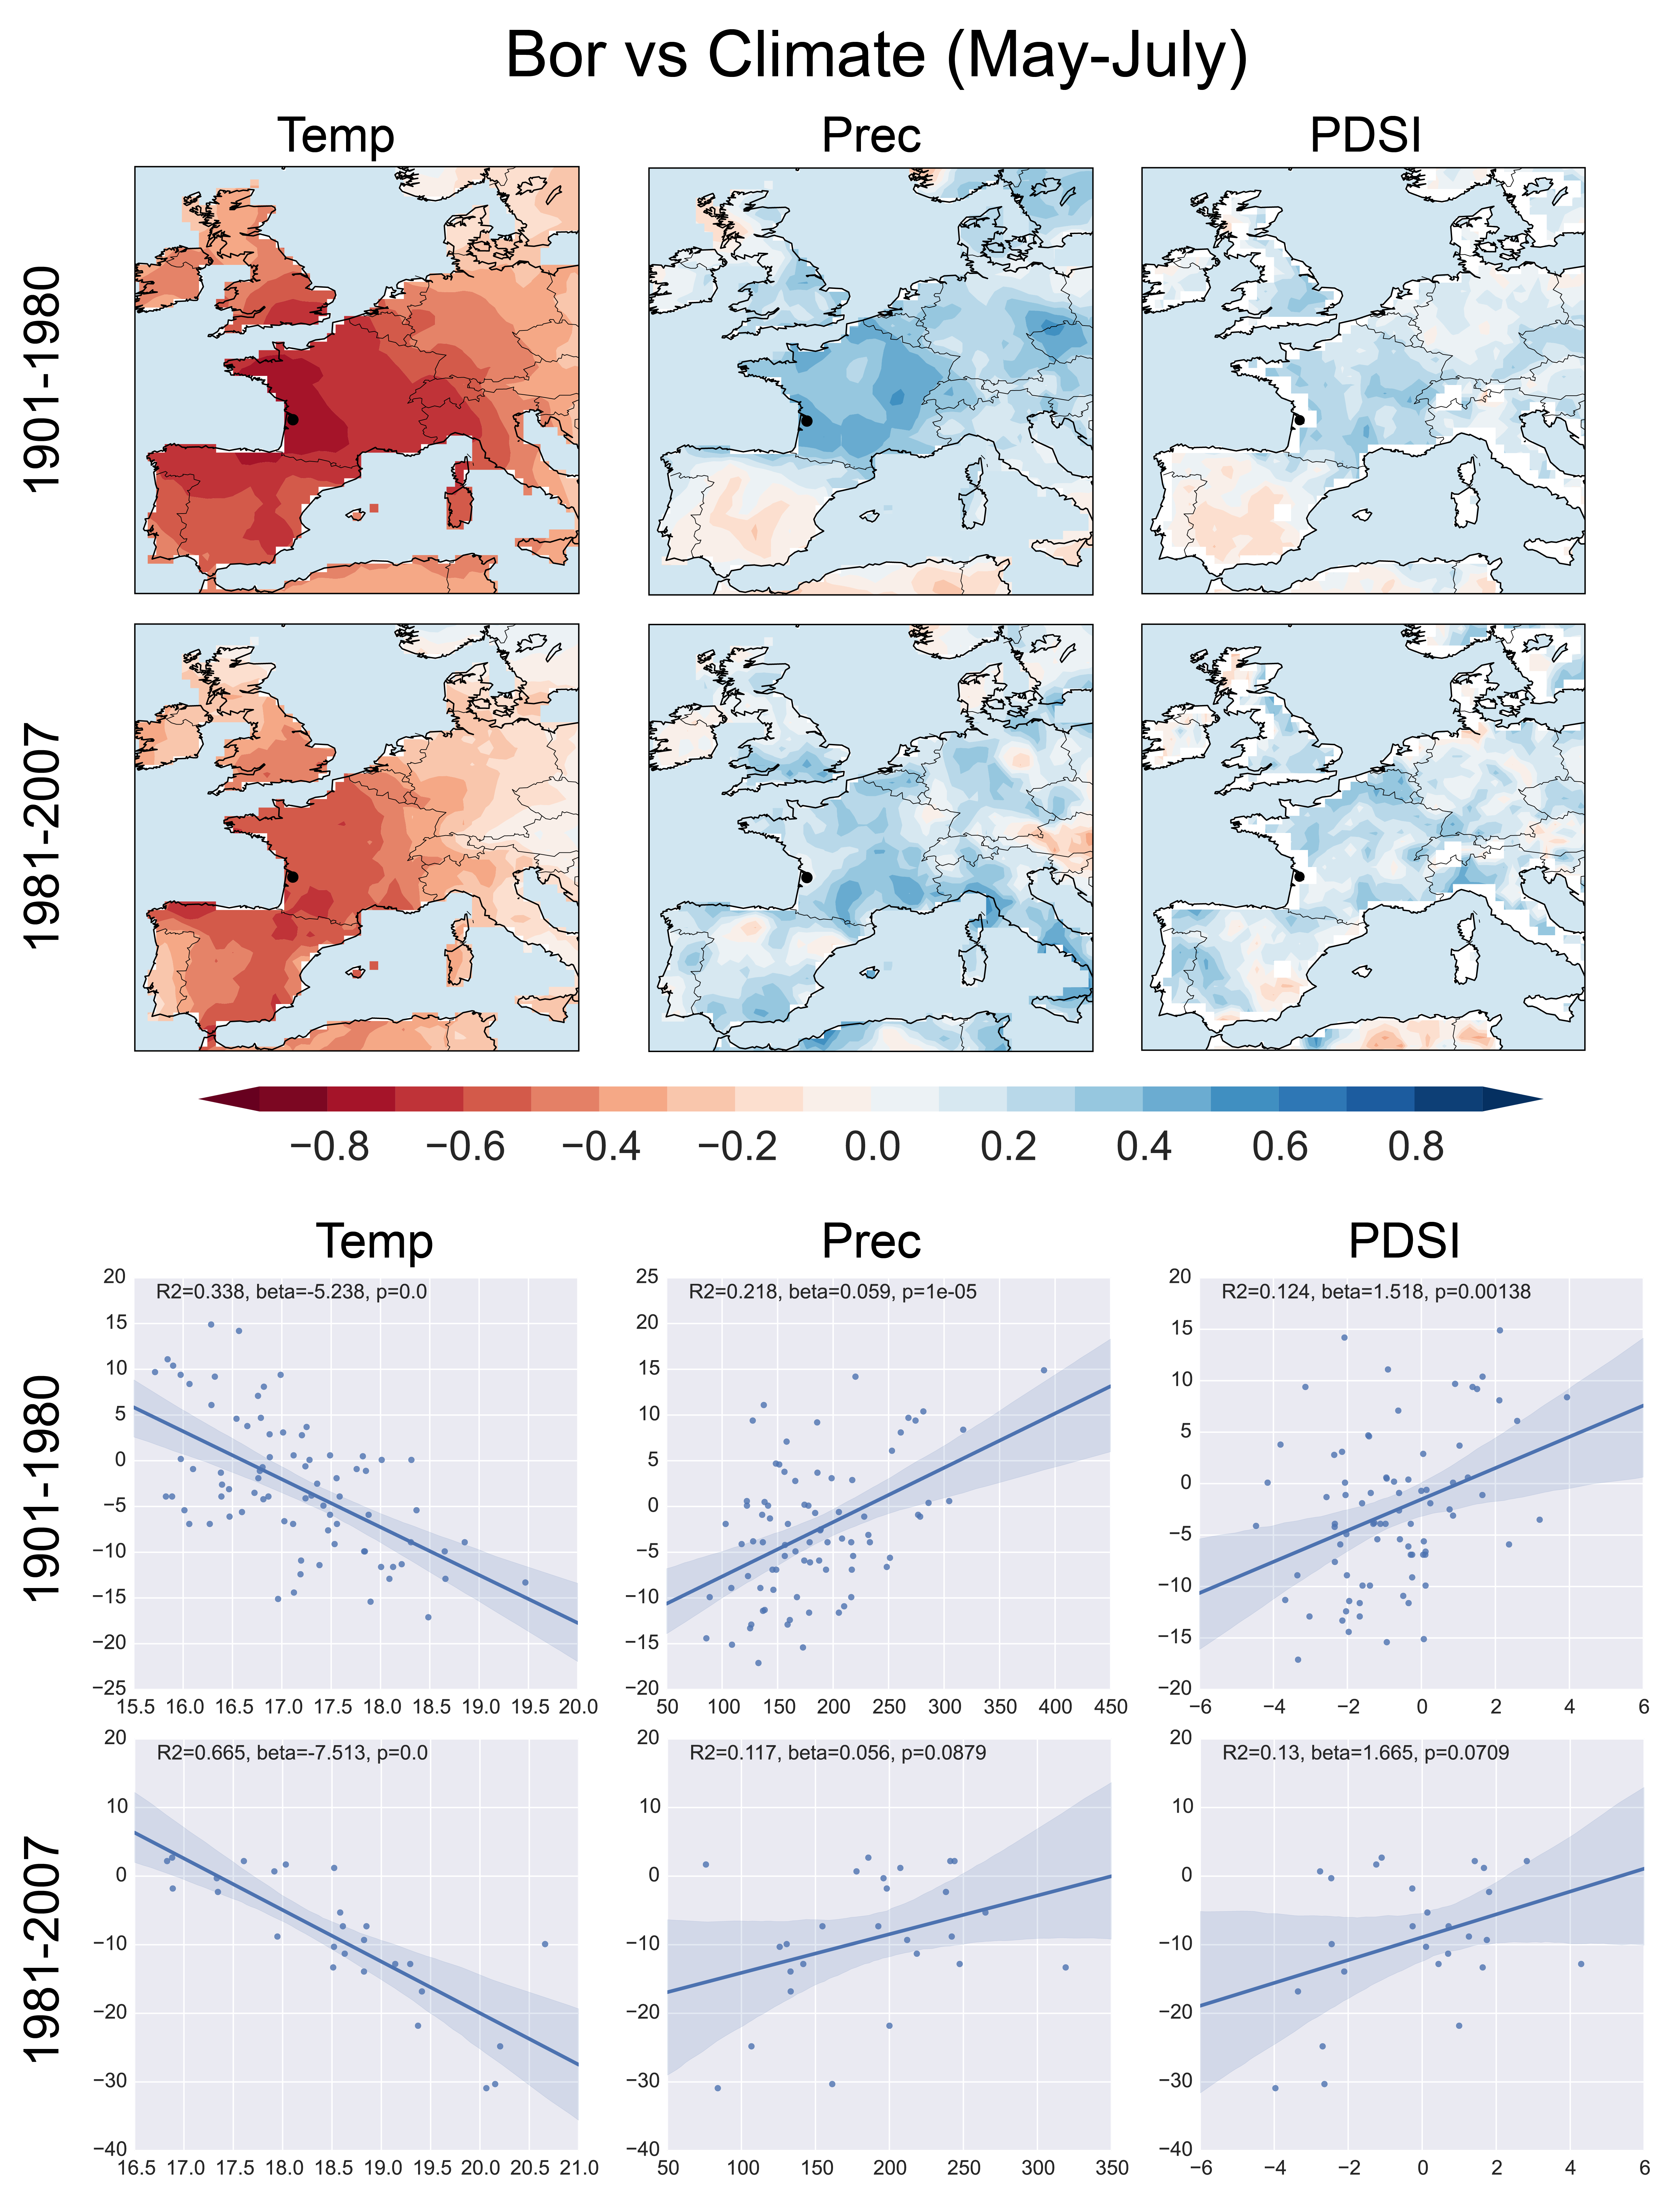
\includegraphics[width=.9\columnwidth,scale=2]{SUPP_fig_05_Bor_MJJ_climate_onedeg.png}
\caption{Same as Figure 4, but for Bor.}
\end{figure}

\begin{figure}
\center
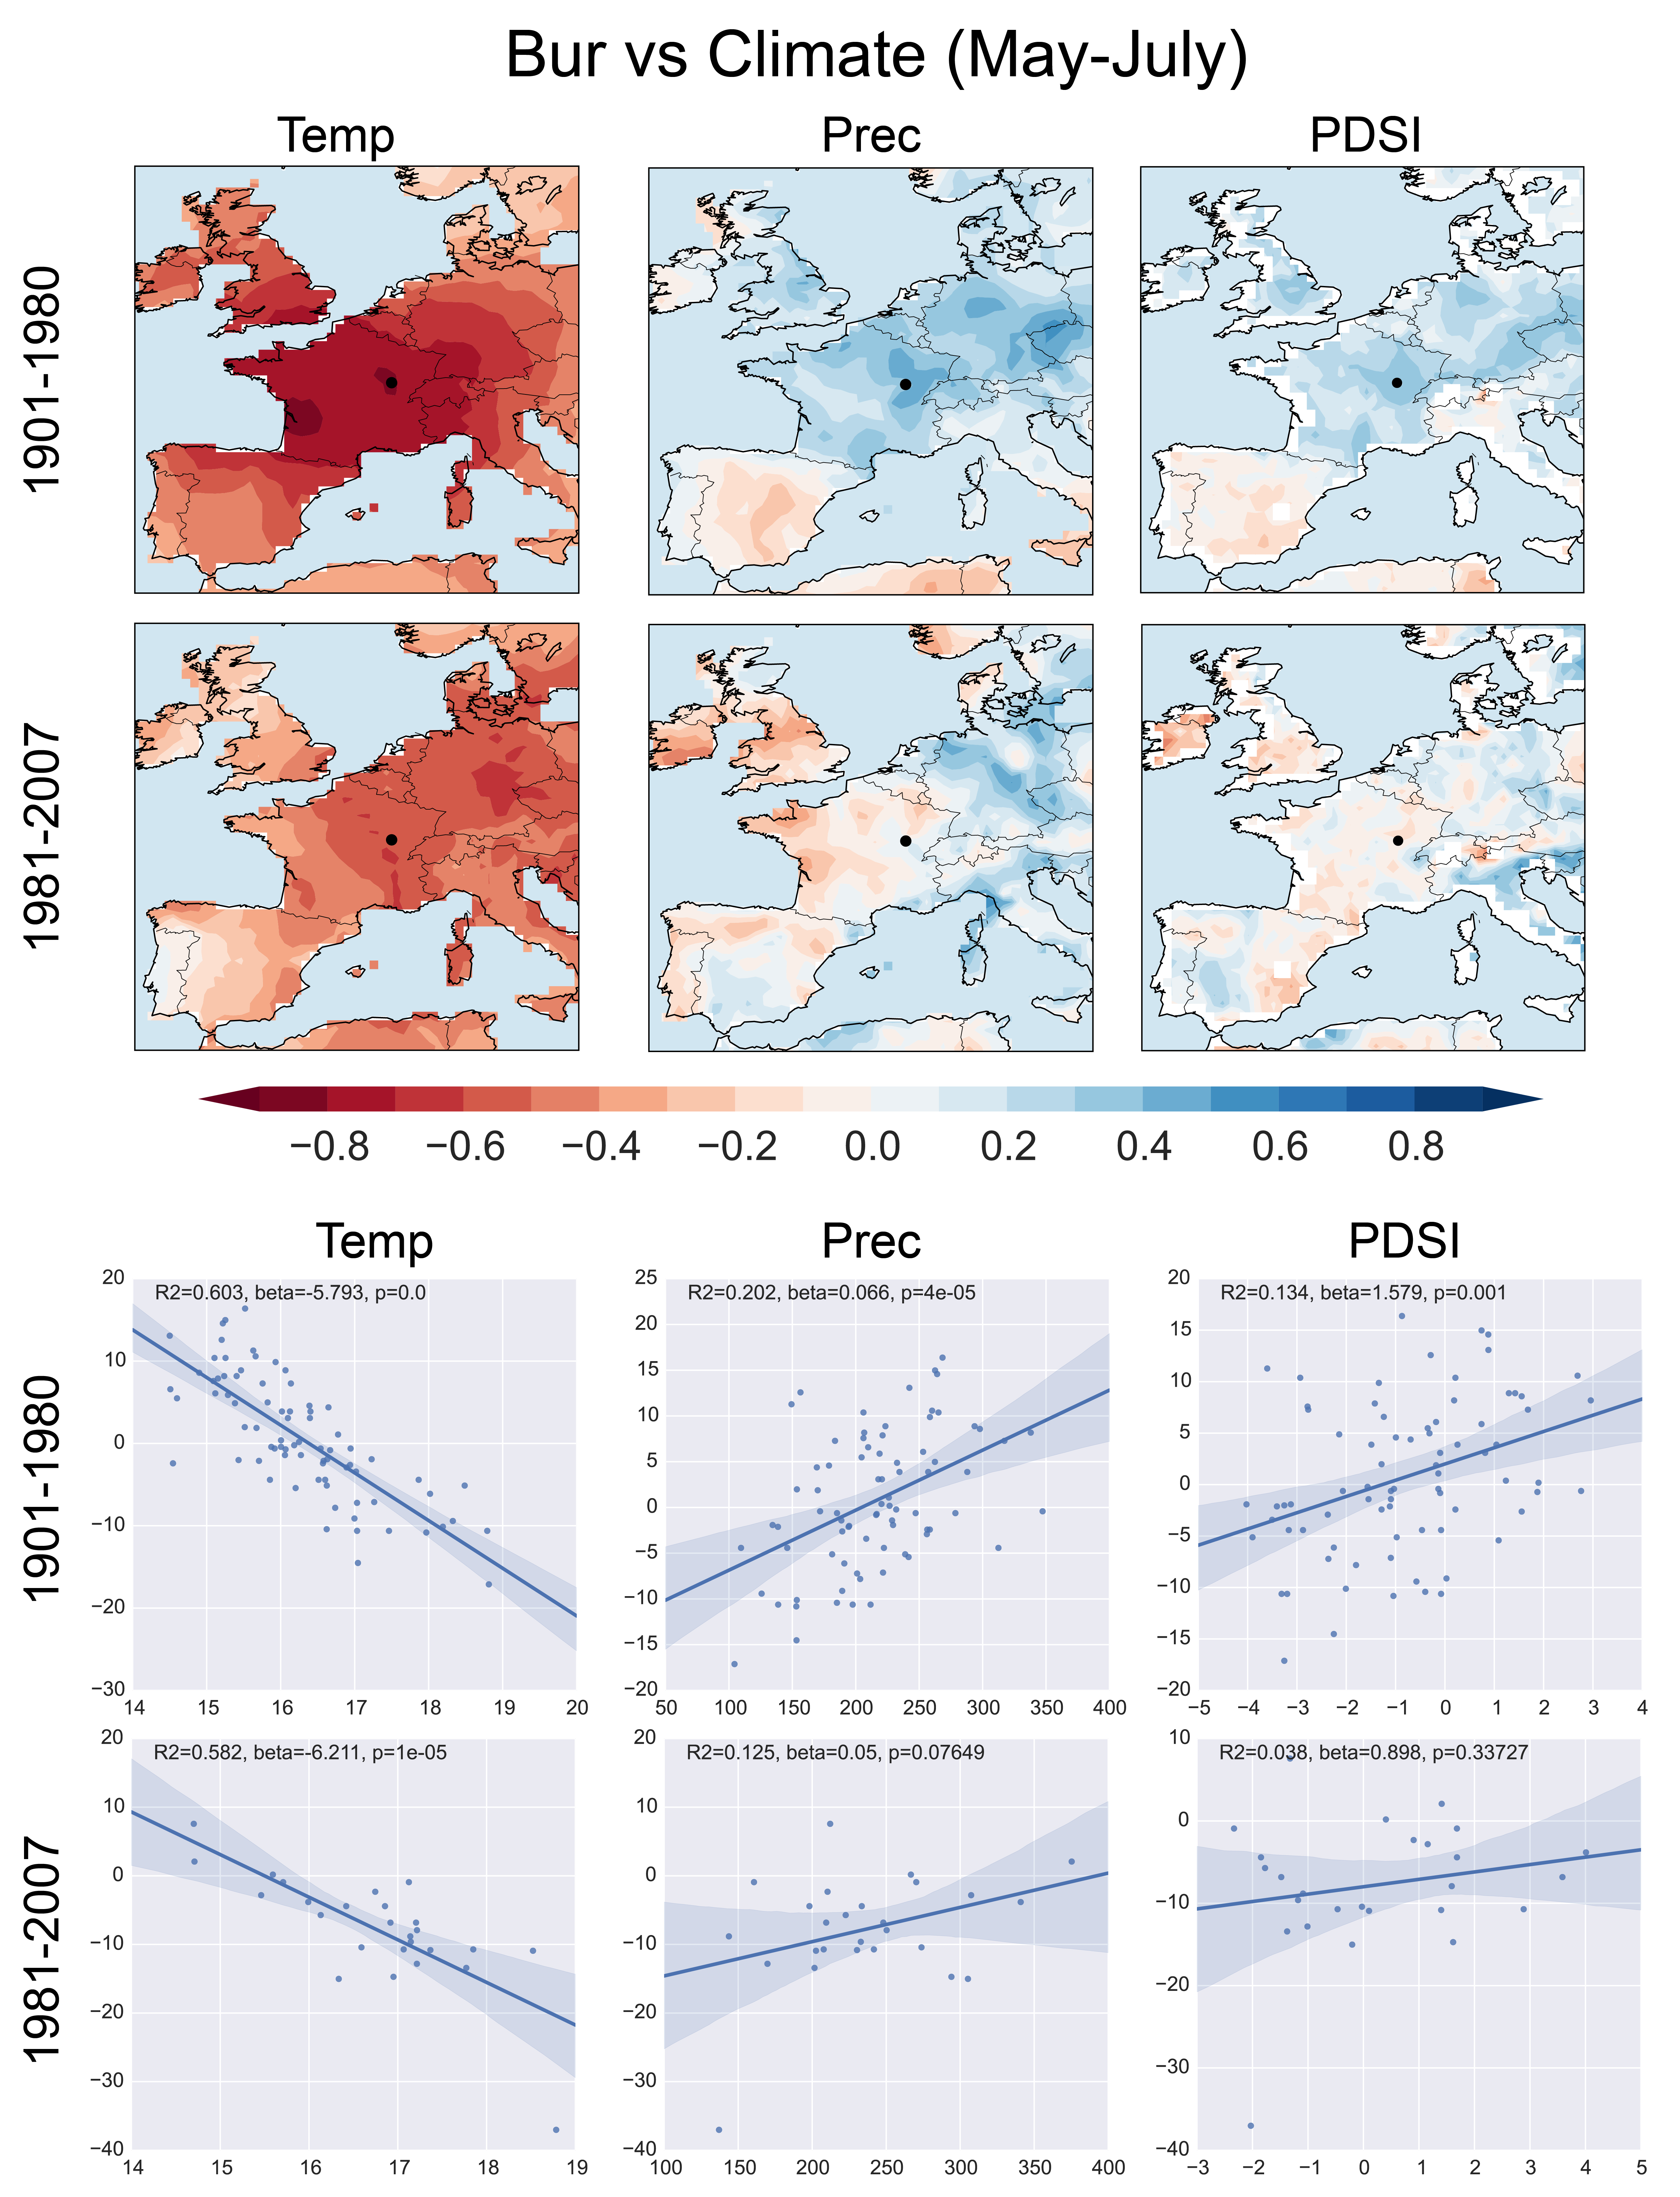
\includegraphics[width=.9\columnwidth,scale=2]{SUPP_fig_06_Bur_MJJ_climate_onedeg.png}
\caption{Same as Figure 4, but for Bur.}
\end{figure}

\begin{figure}
\center
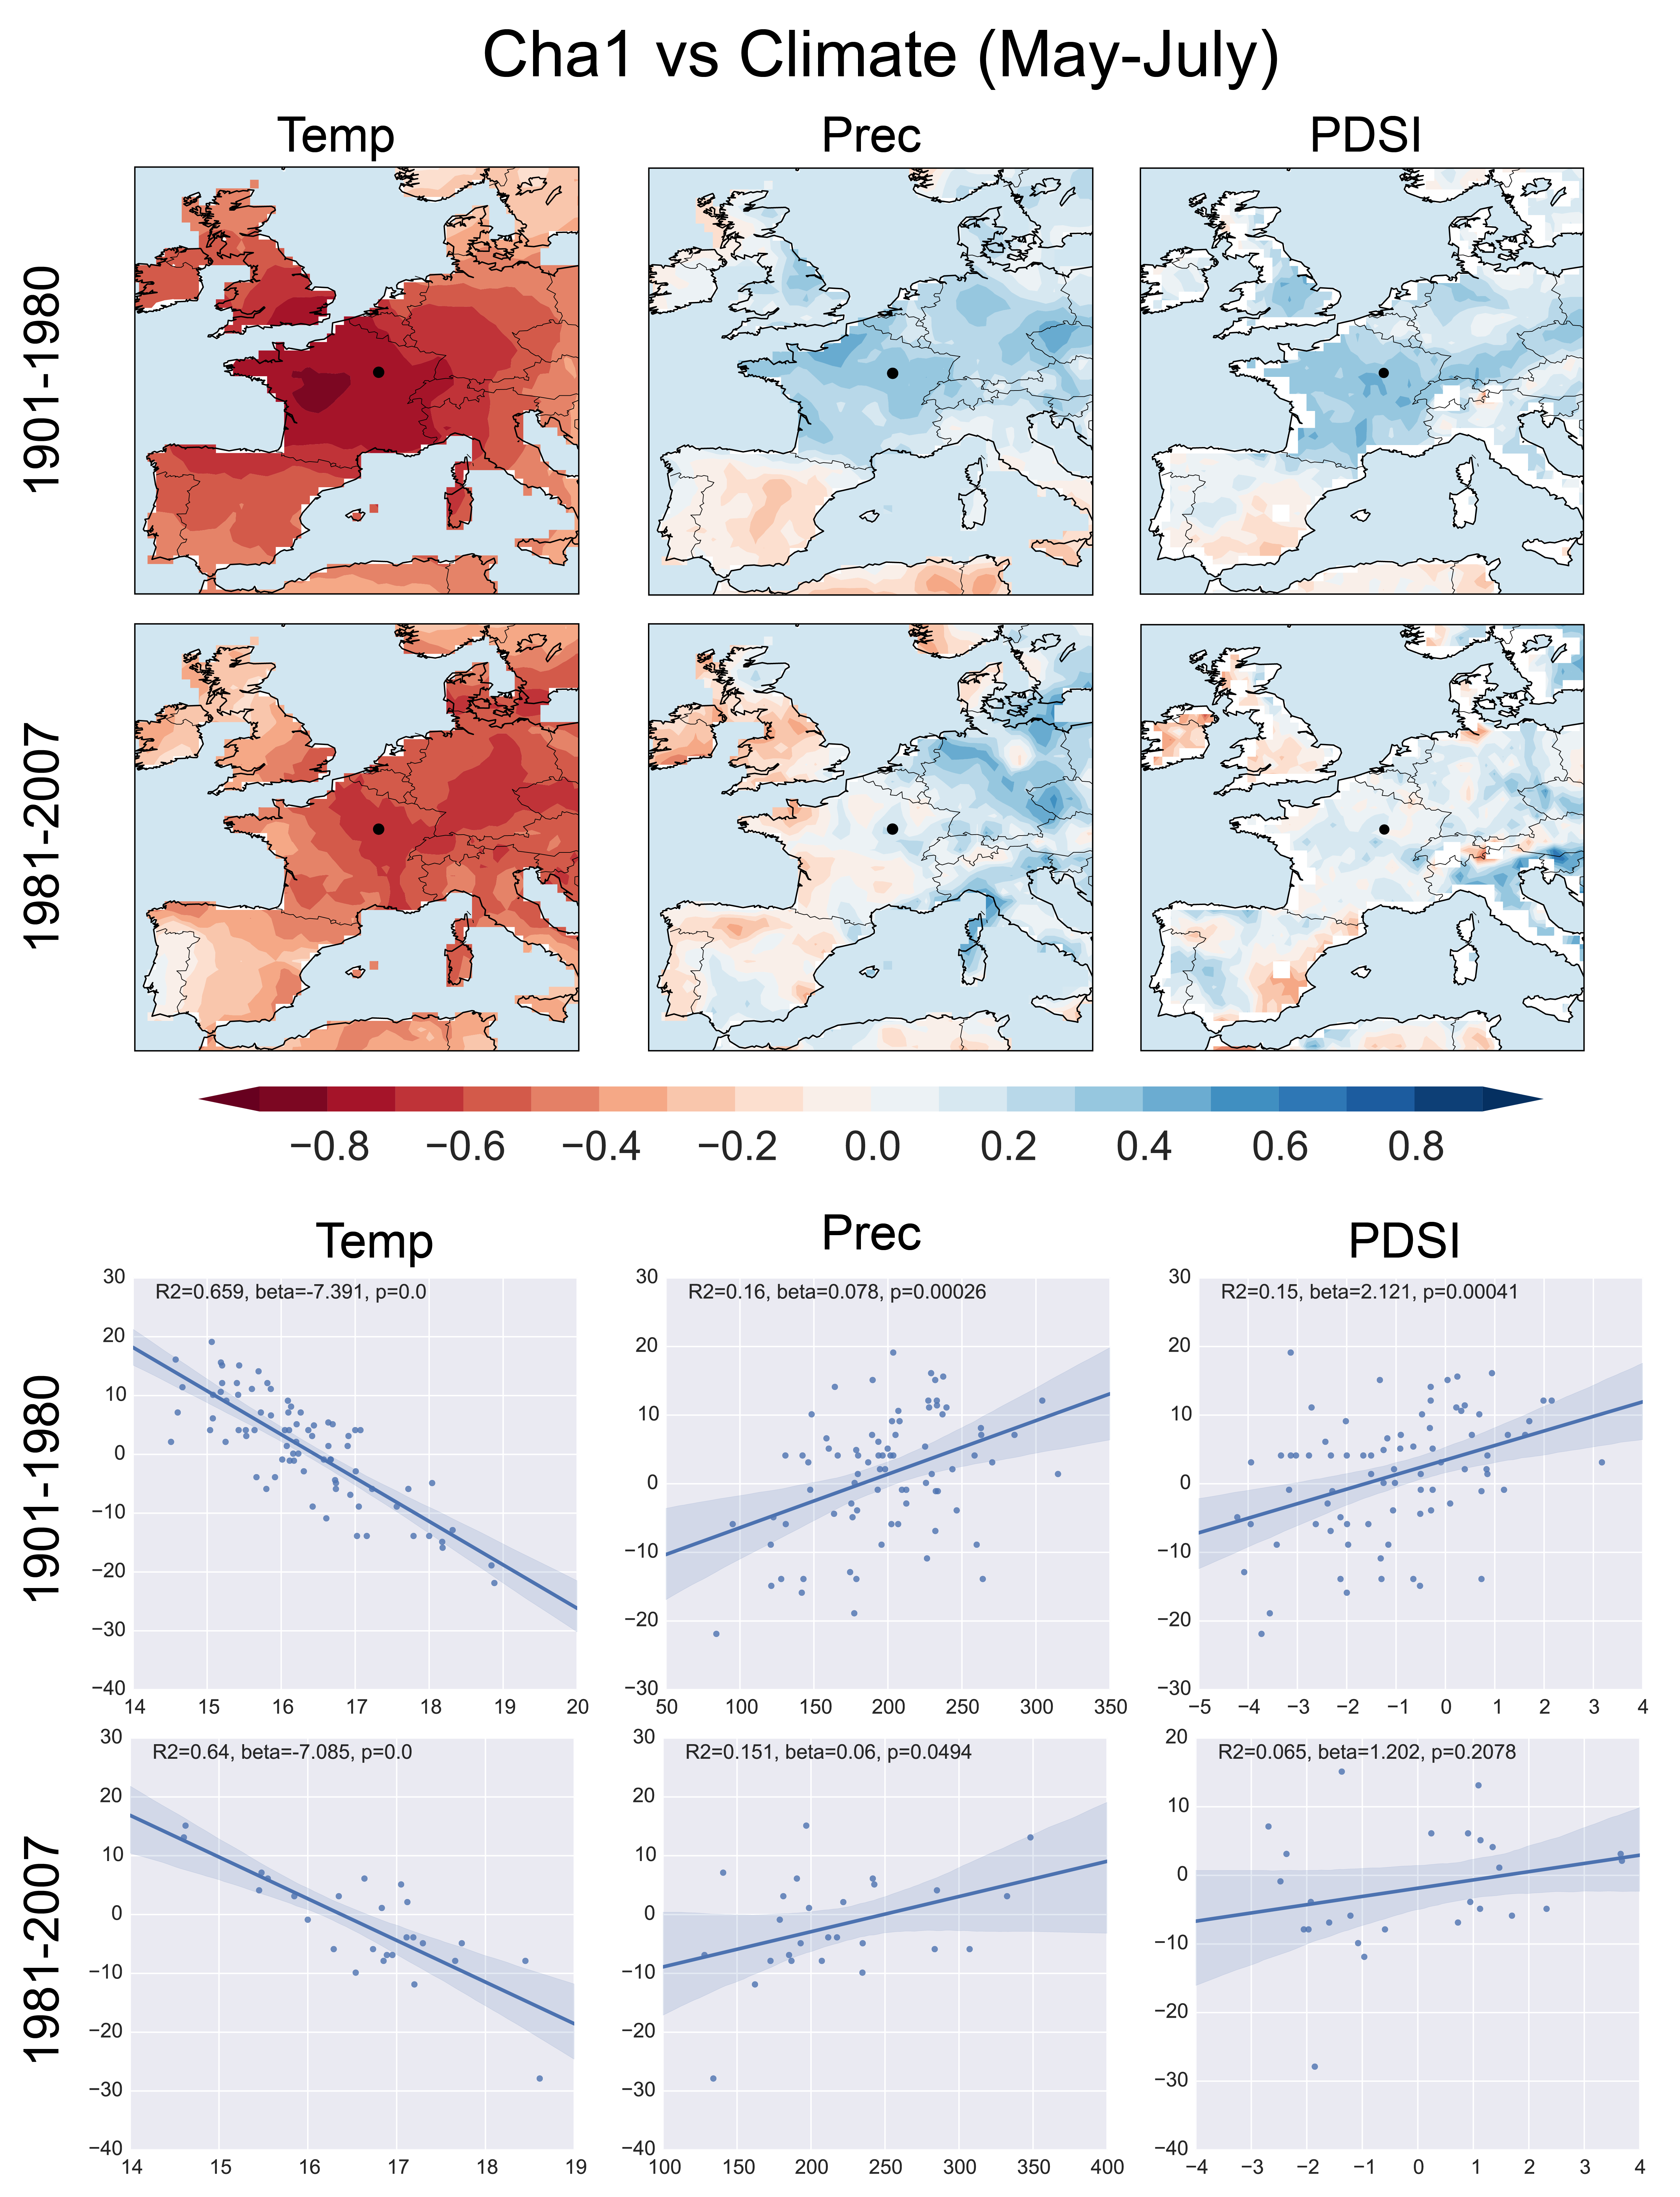
\includegraphics[width=.9\columnwidth,scale=2]{SUPP_fig_07_Cha1_MJJ_climate_onedeg.png}
\caption{Same as Figure 4, but for Cha1.}
\end{figure}

\begin{figure}
\center
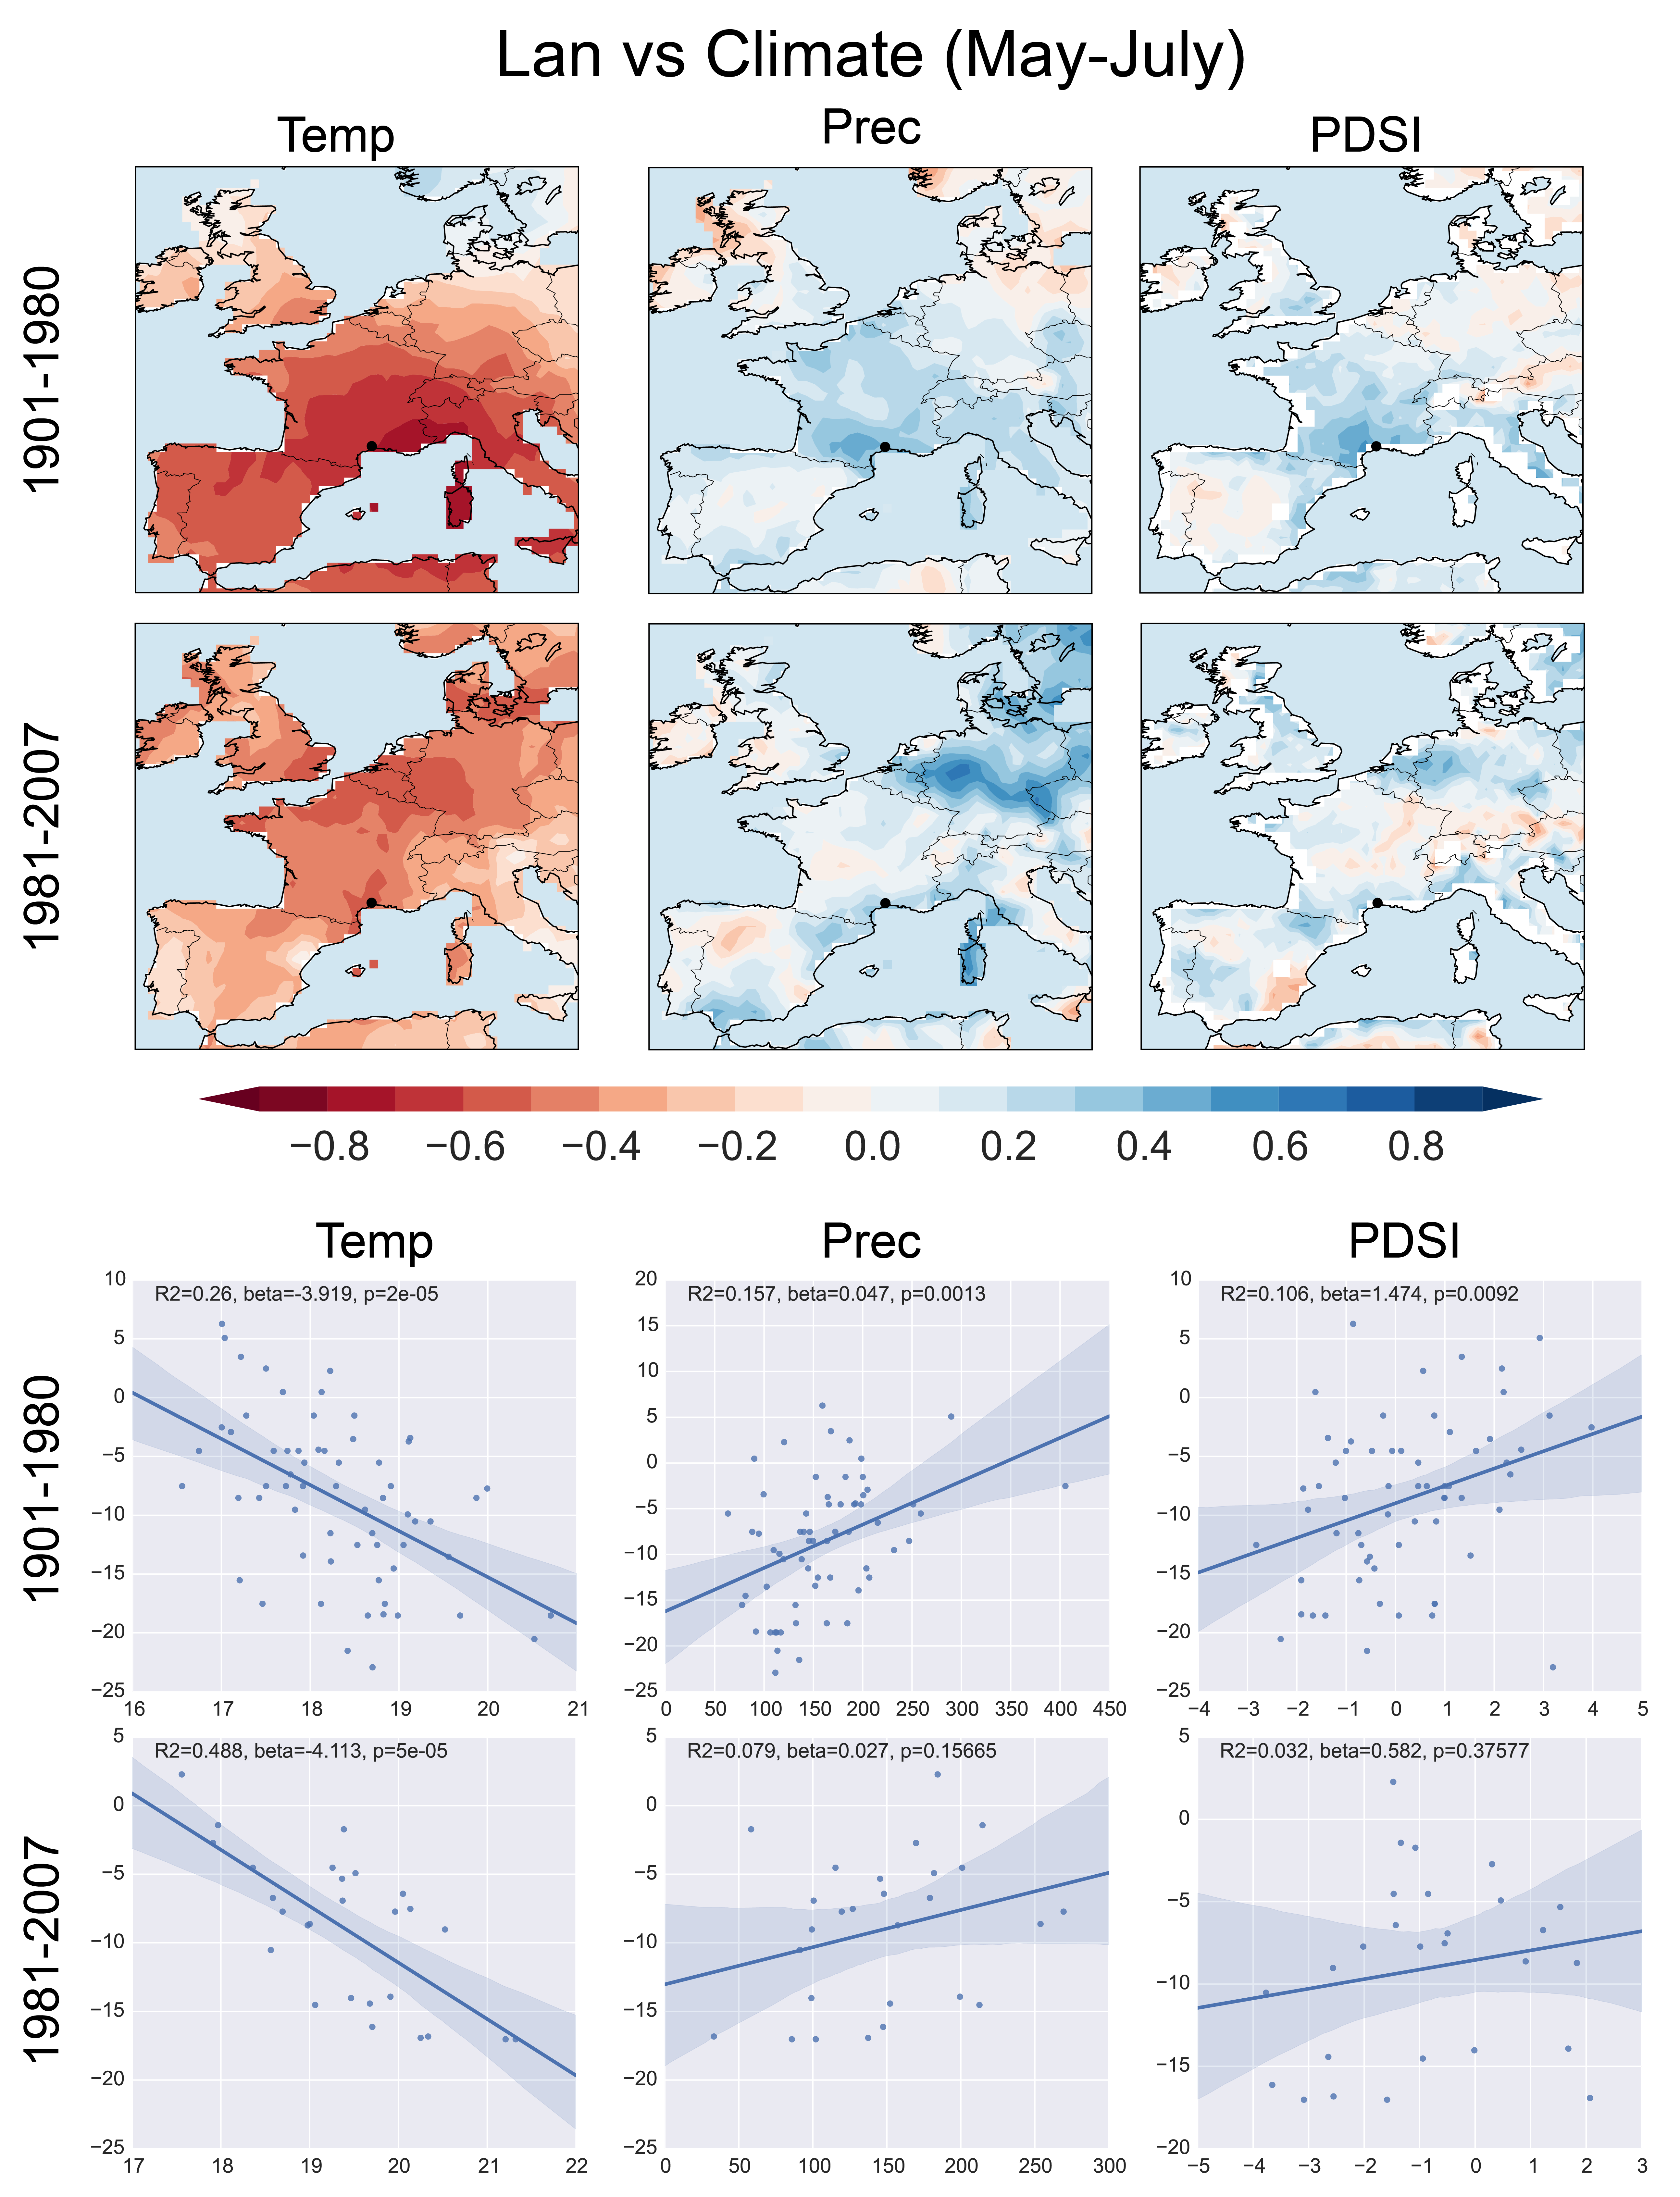
\includegraphics[width=.9\columnwidth,scale=2]{SUPP_fig_08_Lan_MJJ_climate_onedeg.png}
\caption{Same as Figure 4, but for Lan.}
\end{figure}

\begin{figure}
\center
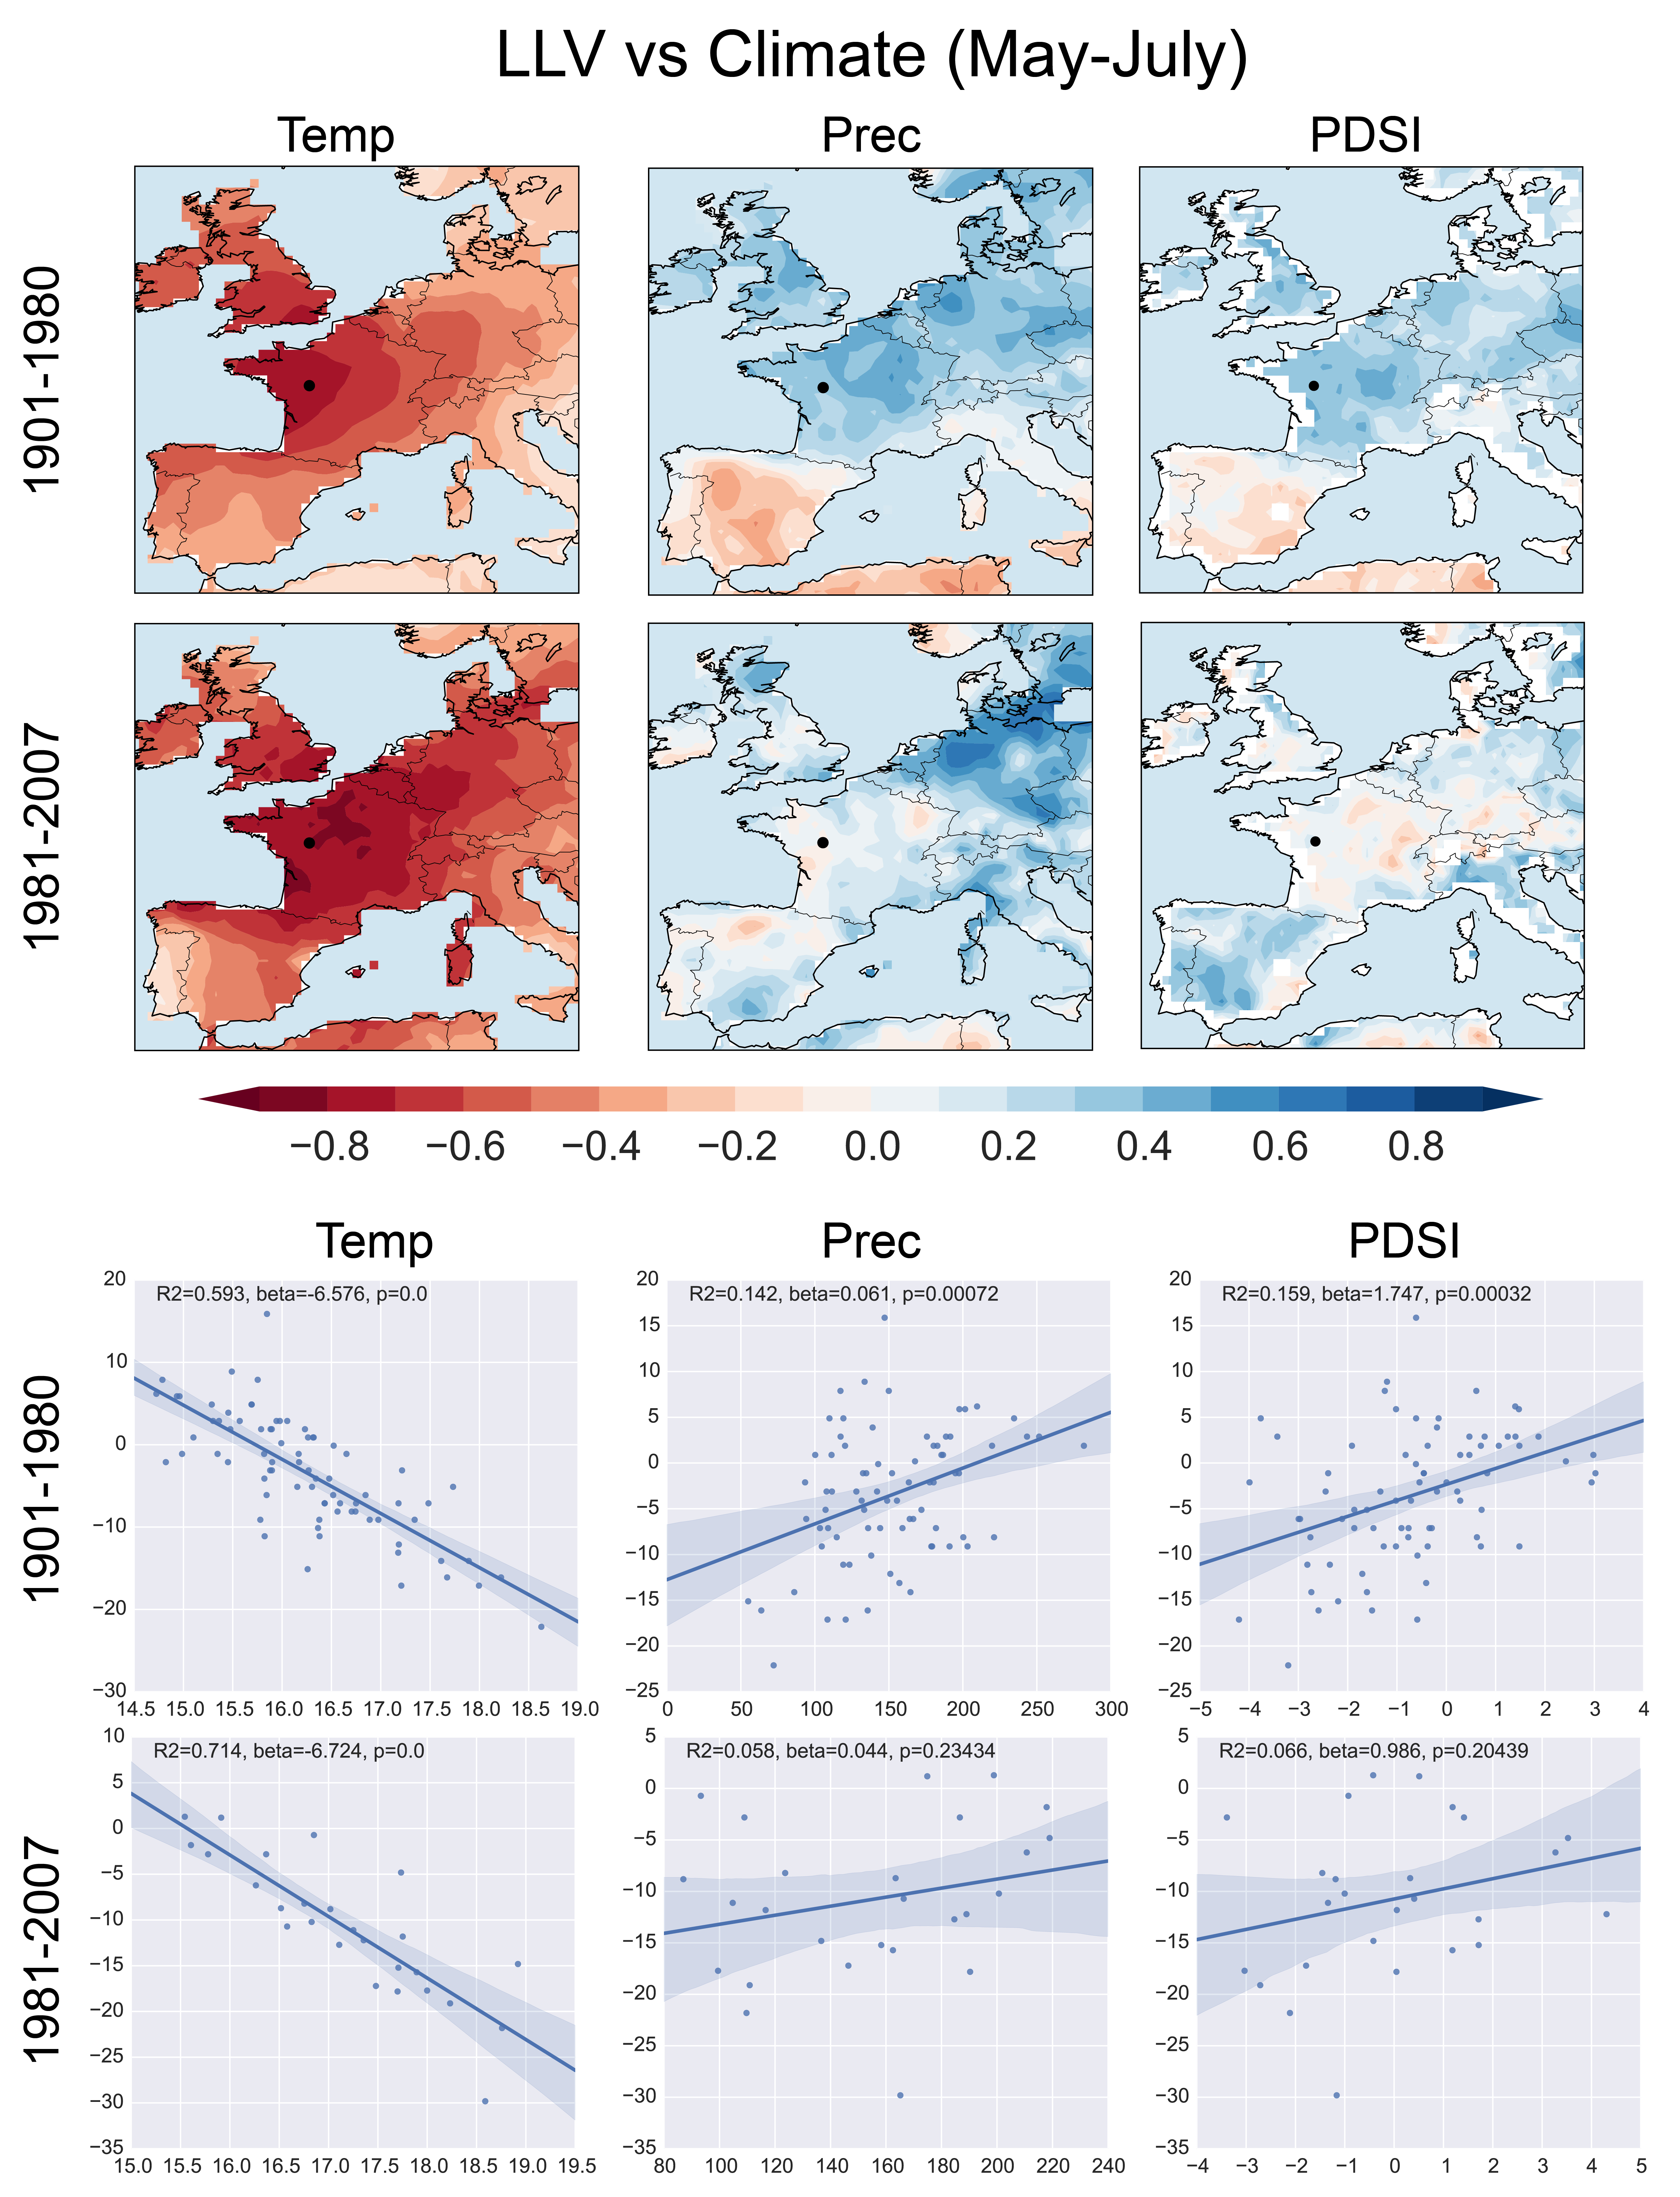
\includegraphics[width=.9\columnwidth,scale=2]{SUPP_fig_09_LLV_MJJ_climate_onedeg.png}
\caption{Same as Figure 4, but for LLV.}
\end{figure}

\begin{figure}
\center
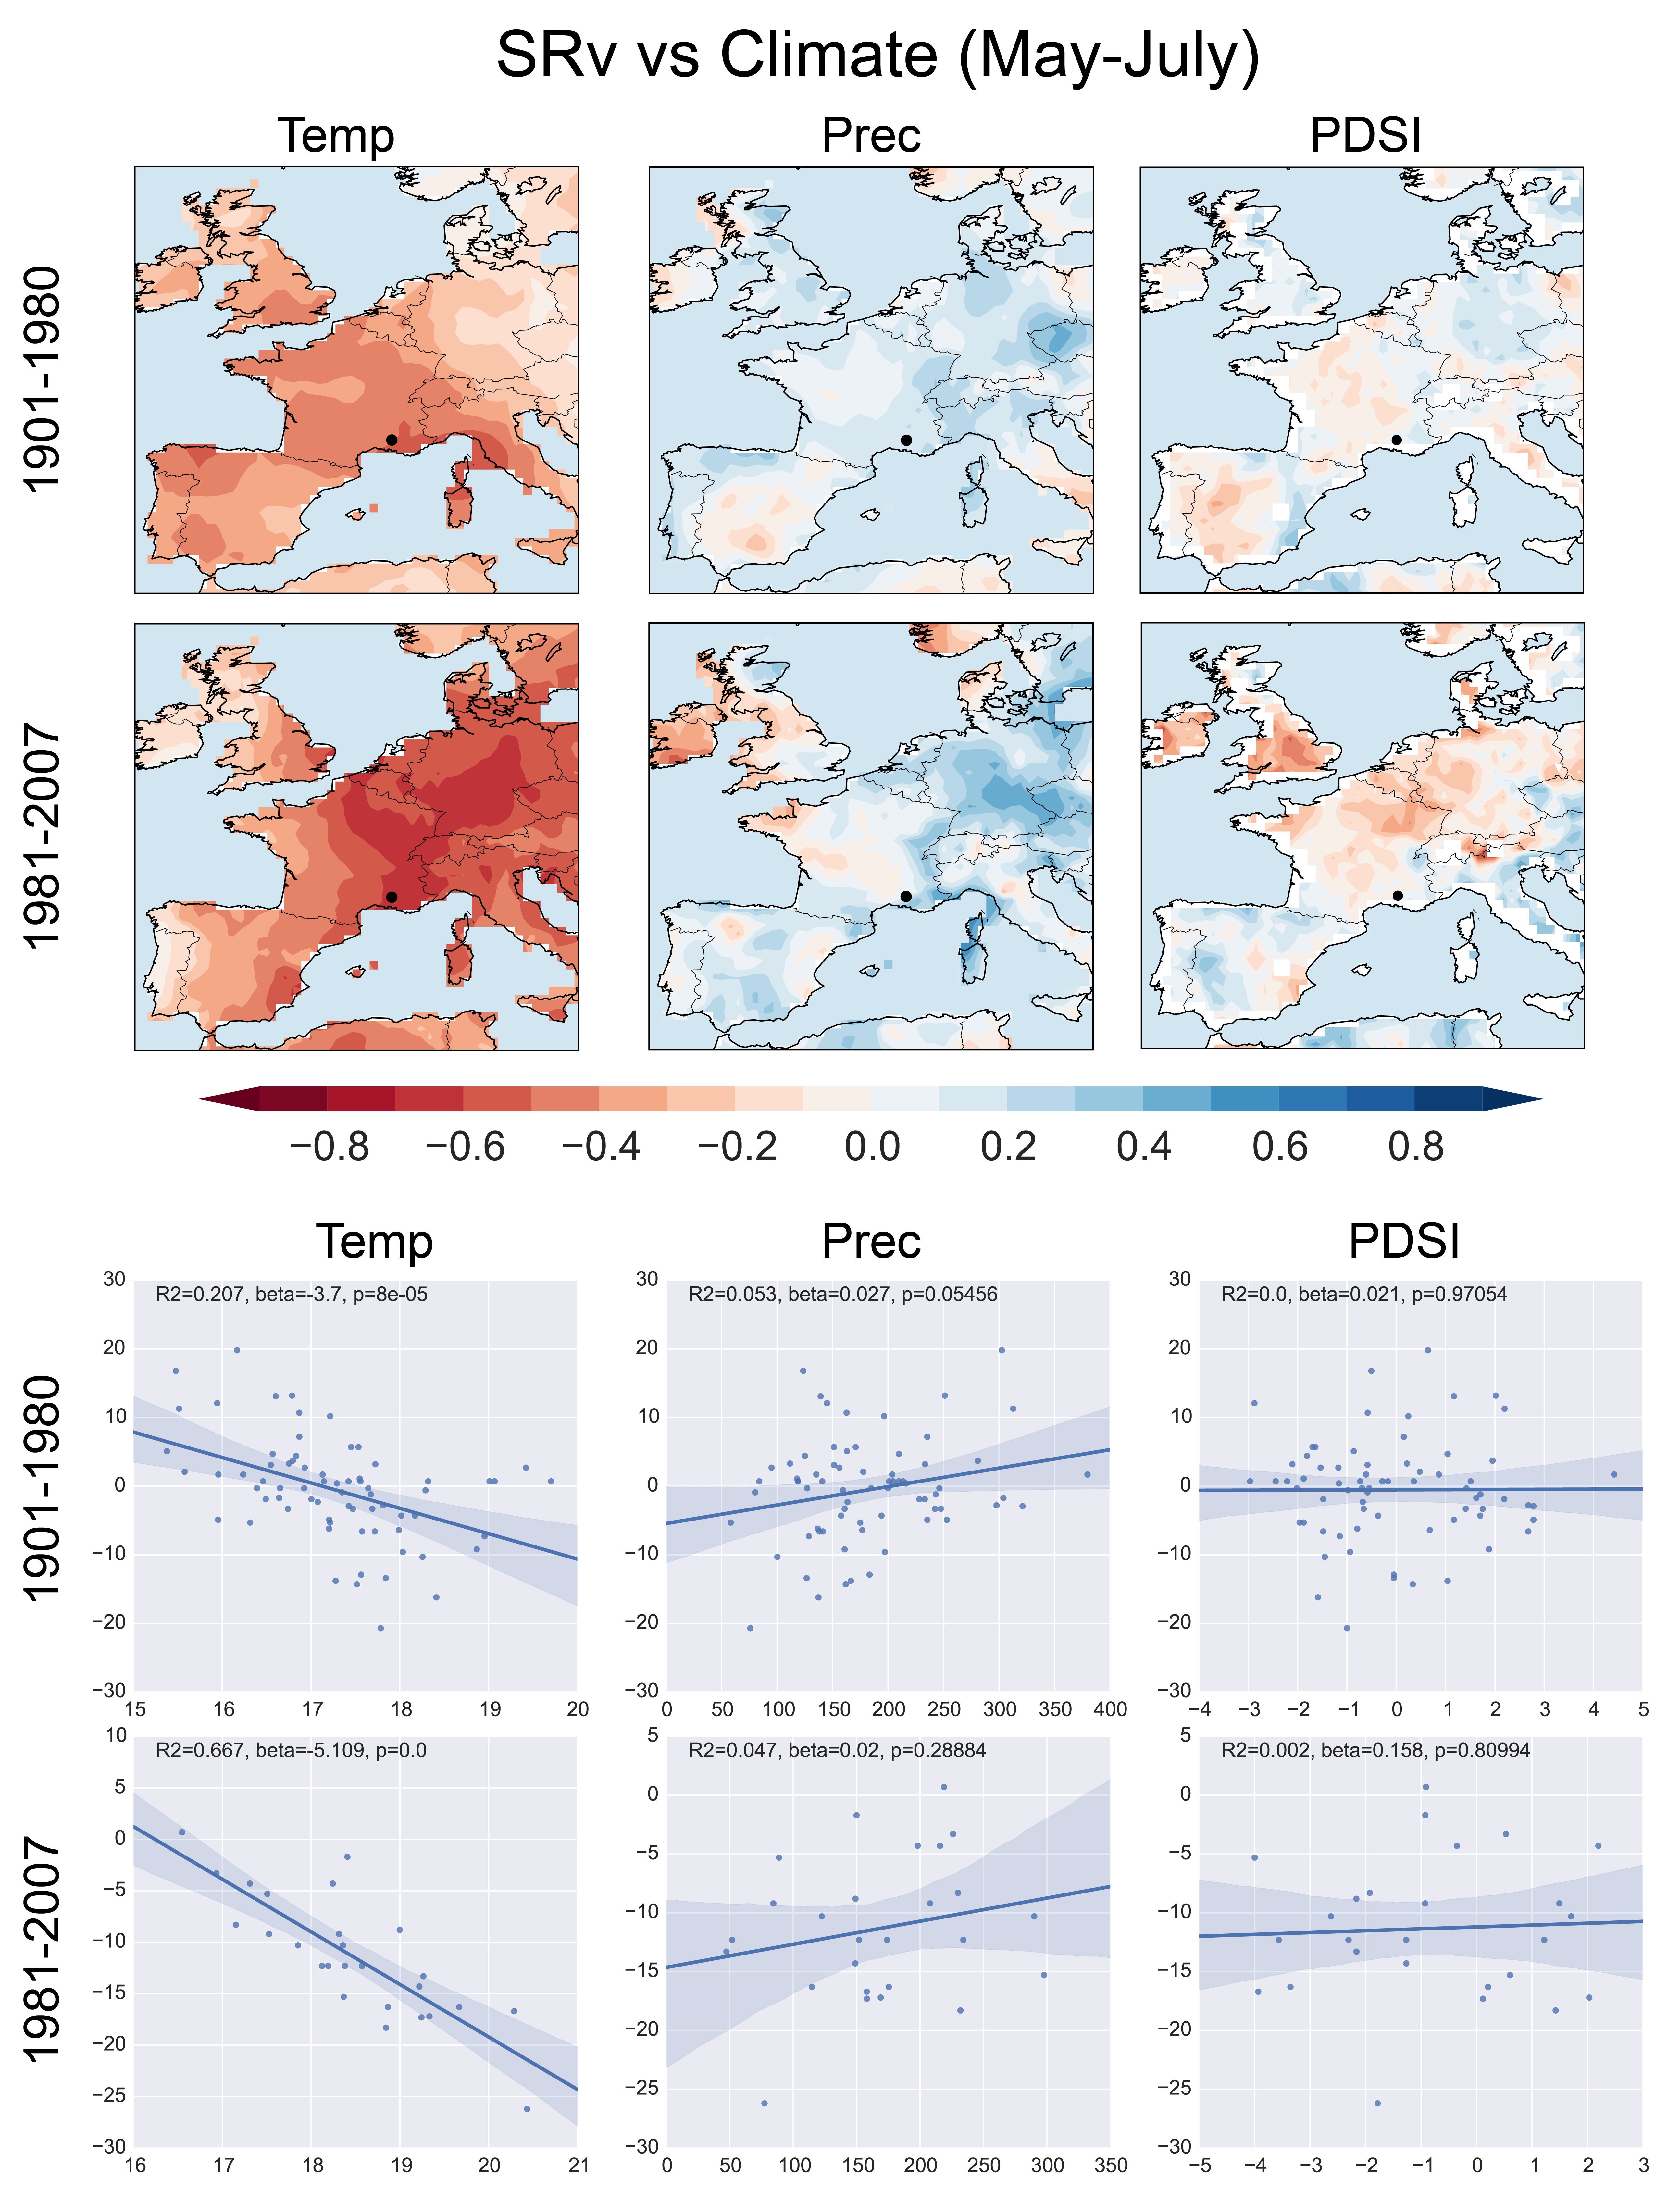
\includegraphics[width=.9\columnwidth,scale=2]{SUPP_fig_10_SRv_MJJ_climate_onedeg.png}
\caption{Same as Figure 4, but for SRv.}
\end{figure}

\begin{figure}
\center
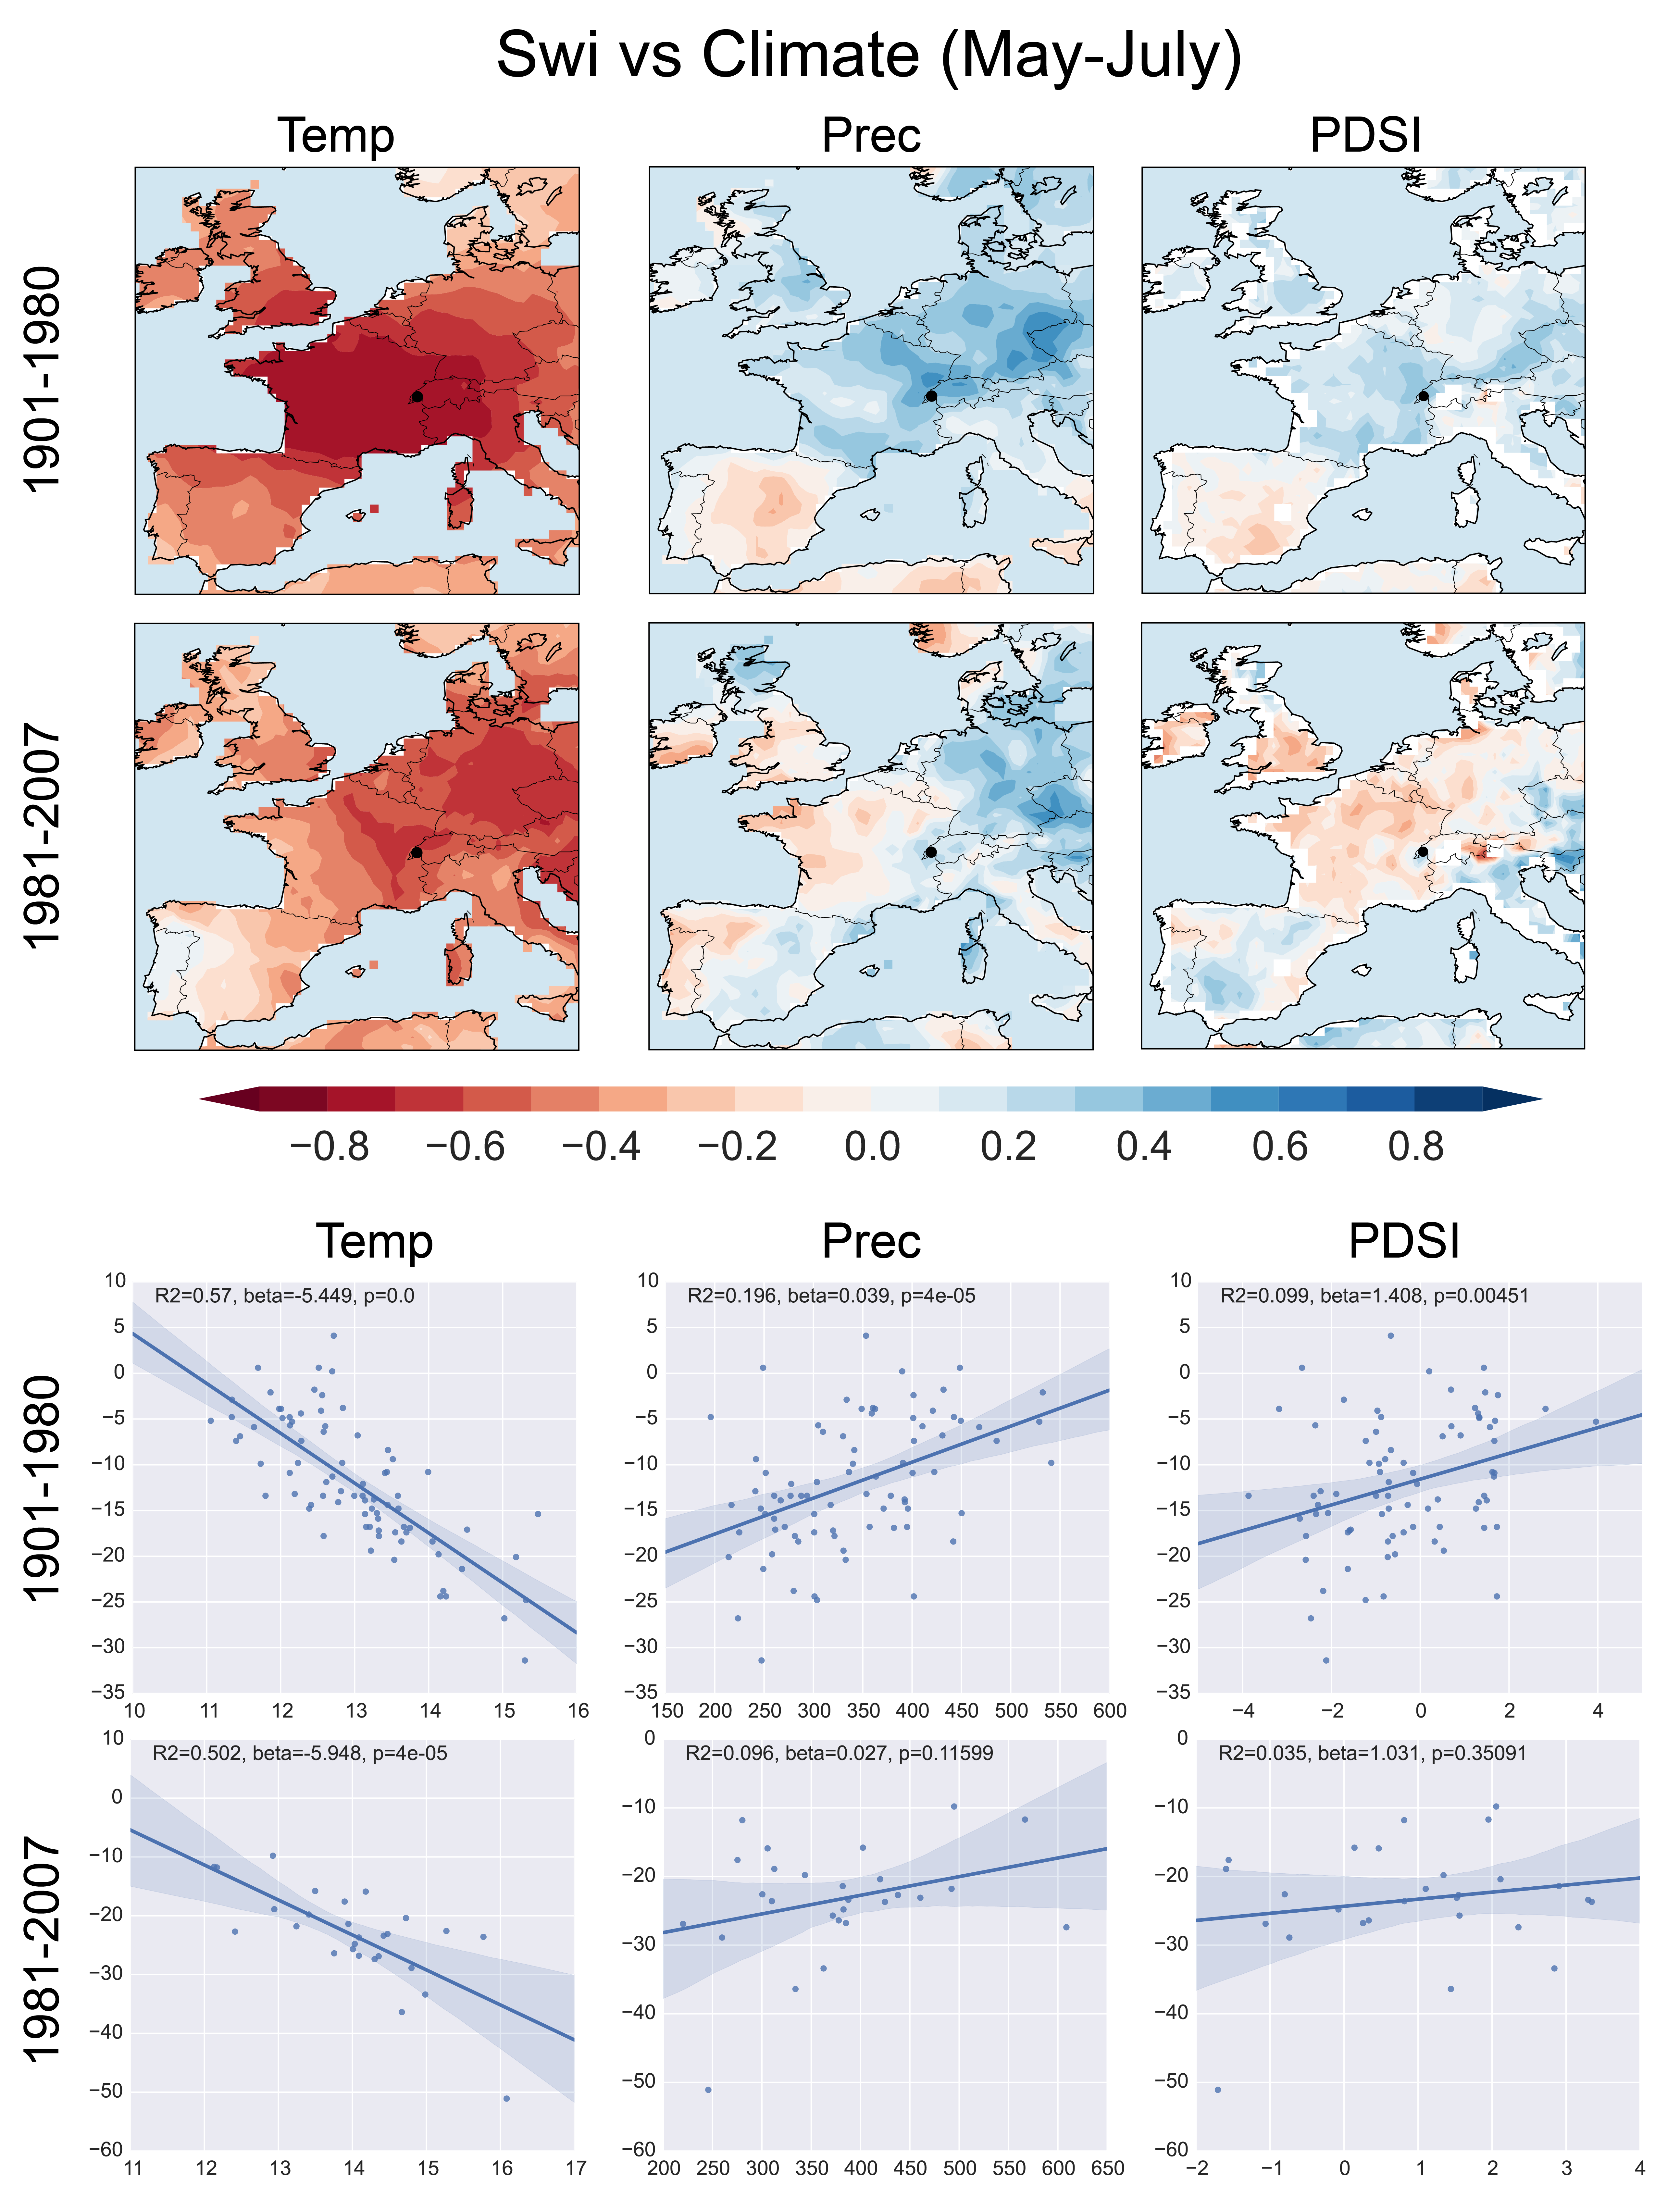
\includegraphics[width=.9\columnwidth,scale=2]{SUPP_fig_11_SWi_MJJ_climate_onedeg.png}
\caption{Same as Figure 4, but for SWi.}
\end{figure}

\begin{figure}
\center
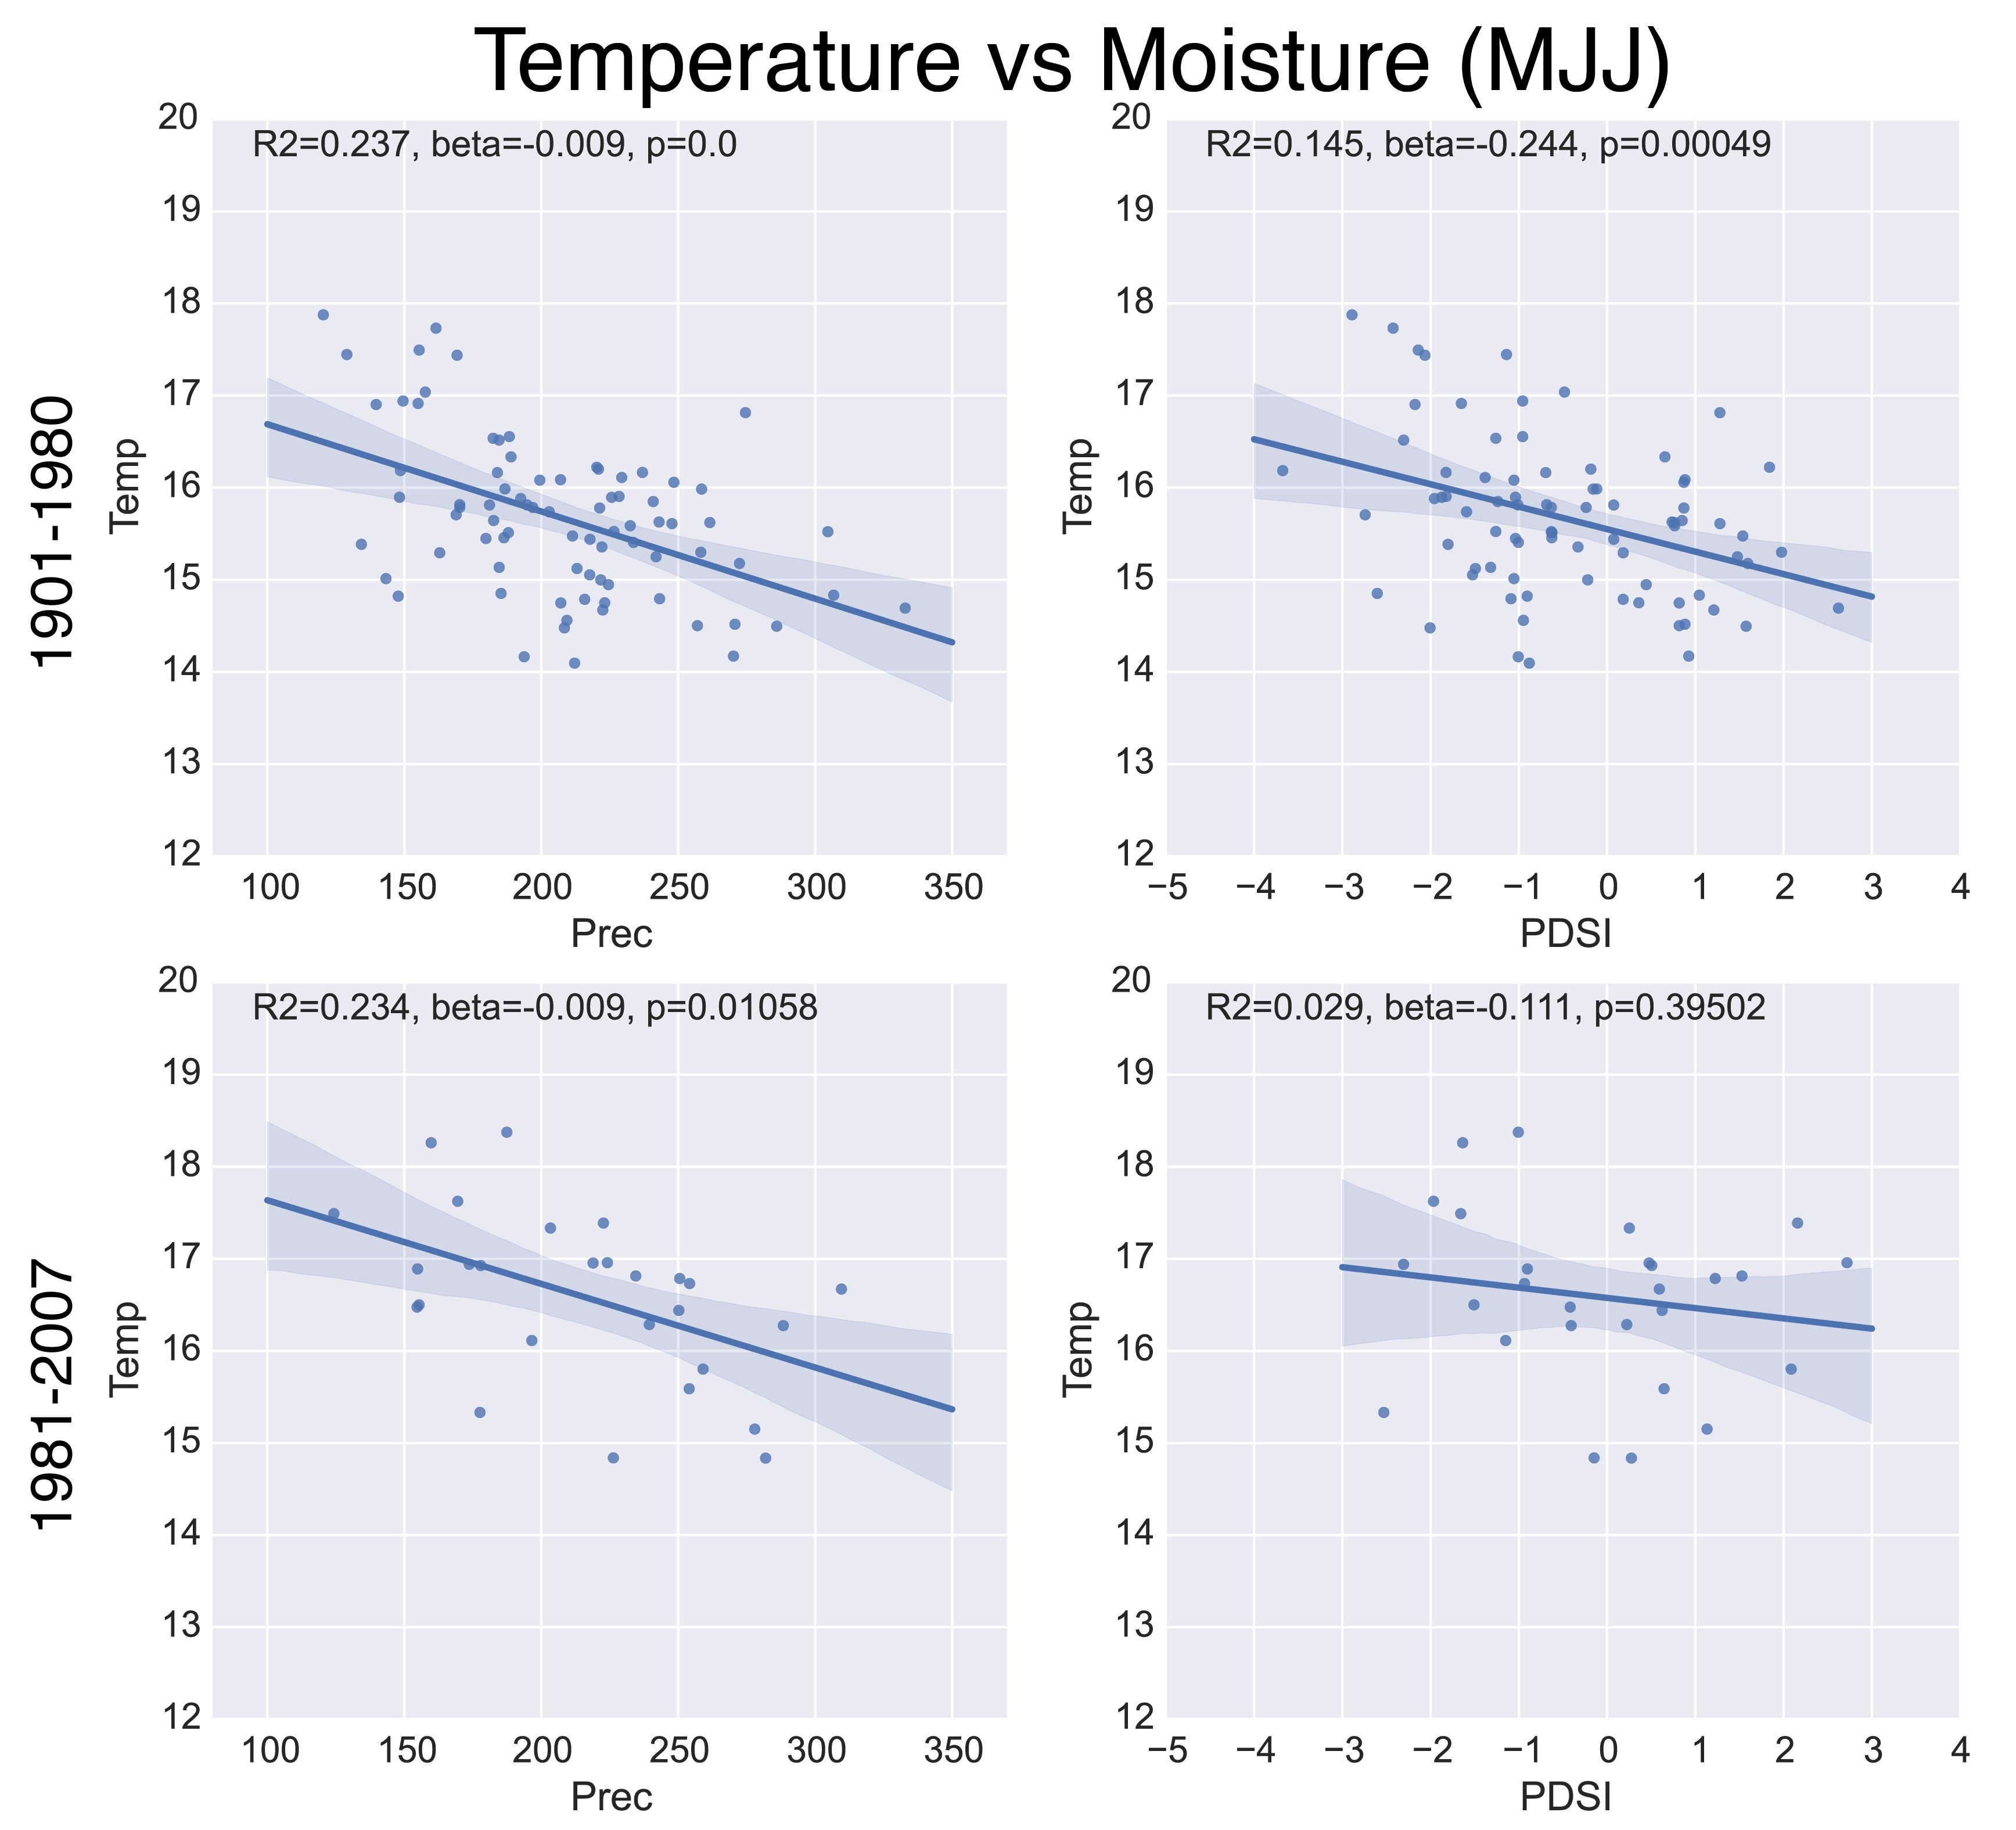
\includegraphics[width=1.0\columnwidth,scale=2]{SUPP_fig_12_temp_vs_moist_MJJ.png}
\caption{Temperature versus moisture (precipitation and PDSI) during May-June-July for the GHD-Core region from the CRU 3.21 climate grids for two periods: 1901--1980 and 1981--2007. Temperature during MJJ has a significant negative relationship with both precipitation and PDSI, indicating the tendency for warmer conditions during drier years. Over the more recent period, the relationship between temperature and PDSI breaks down, but the relationship with precipitation remains largely consistent.}
\end{figure}

\begin{figure}
\center
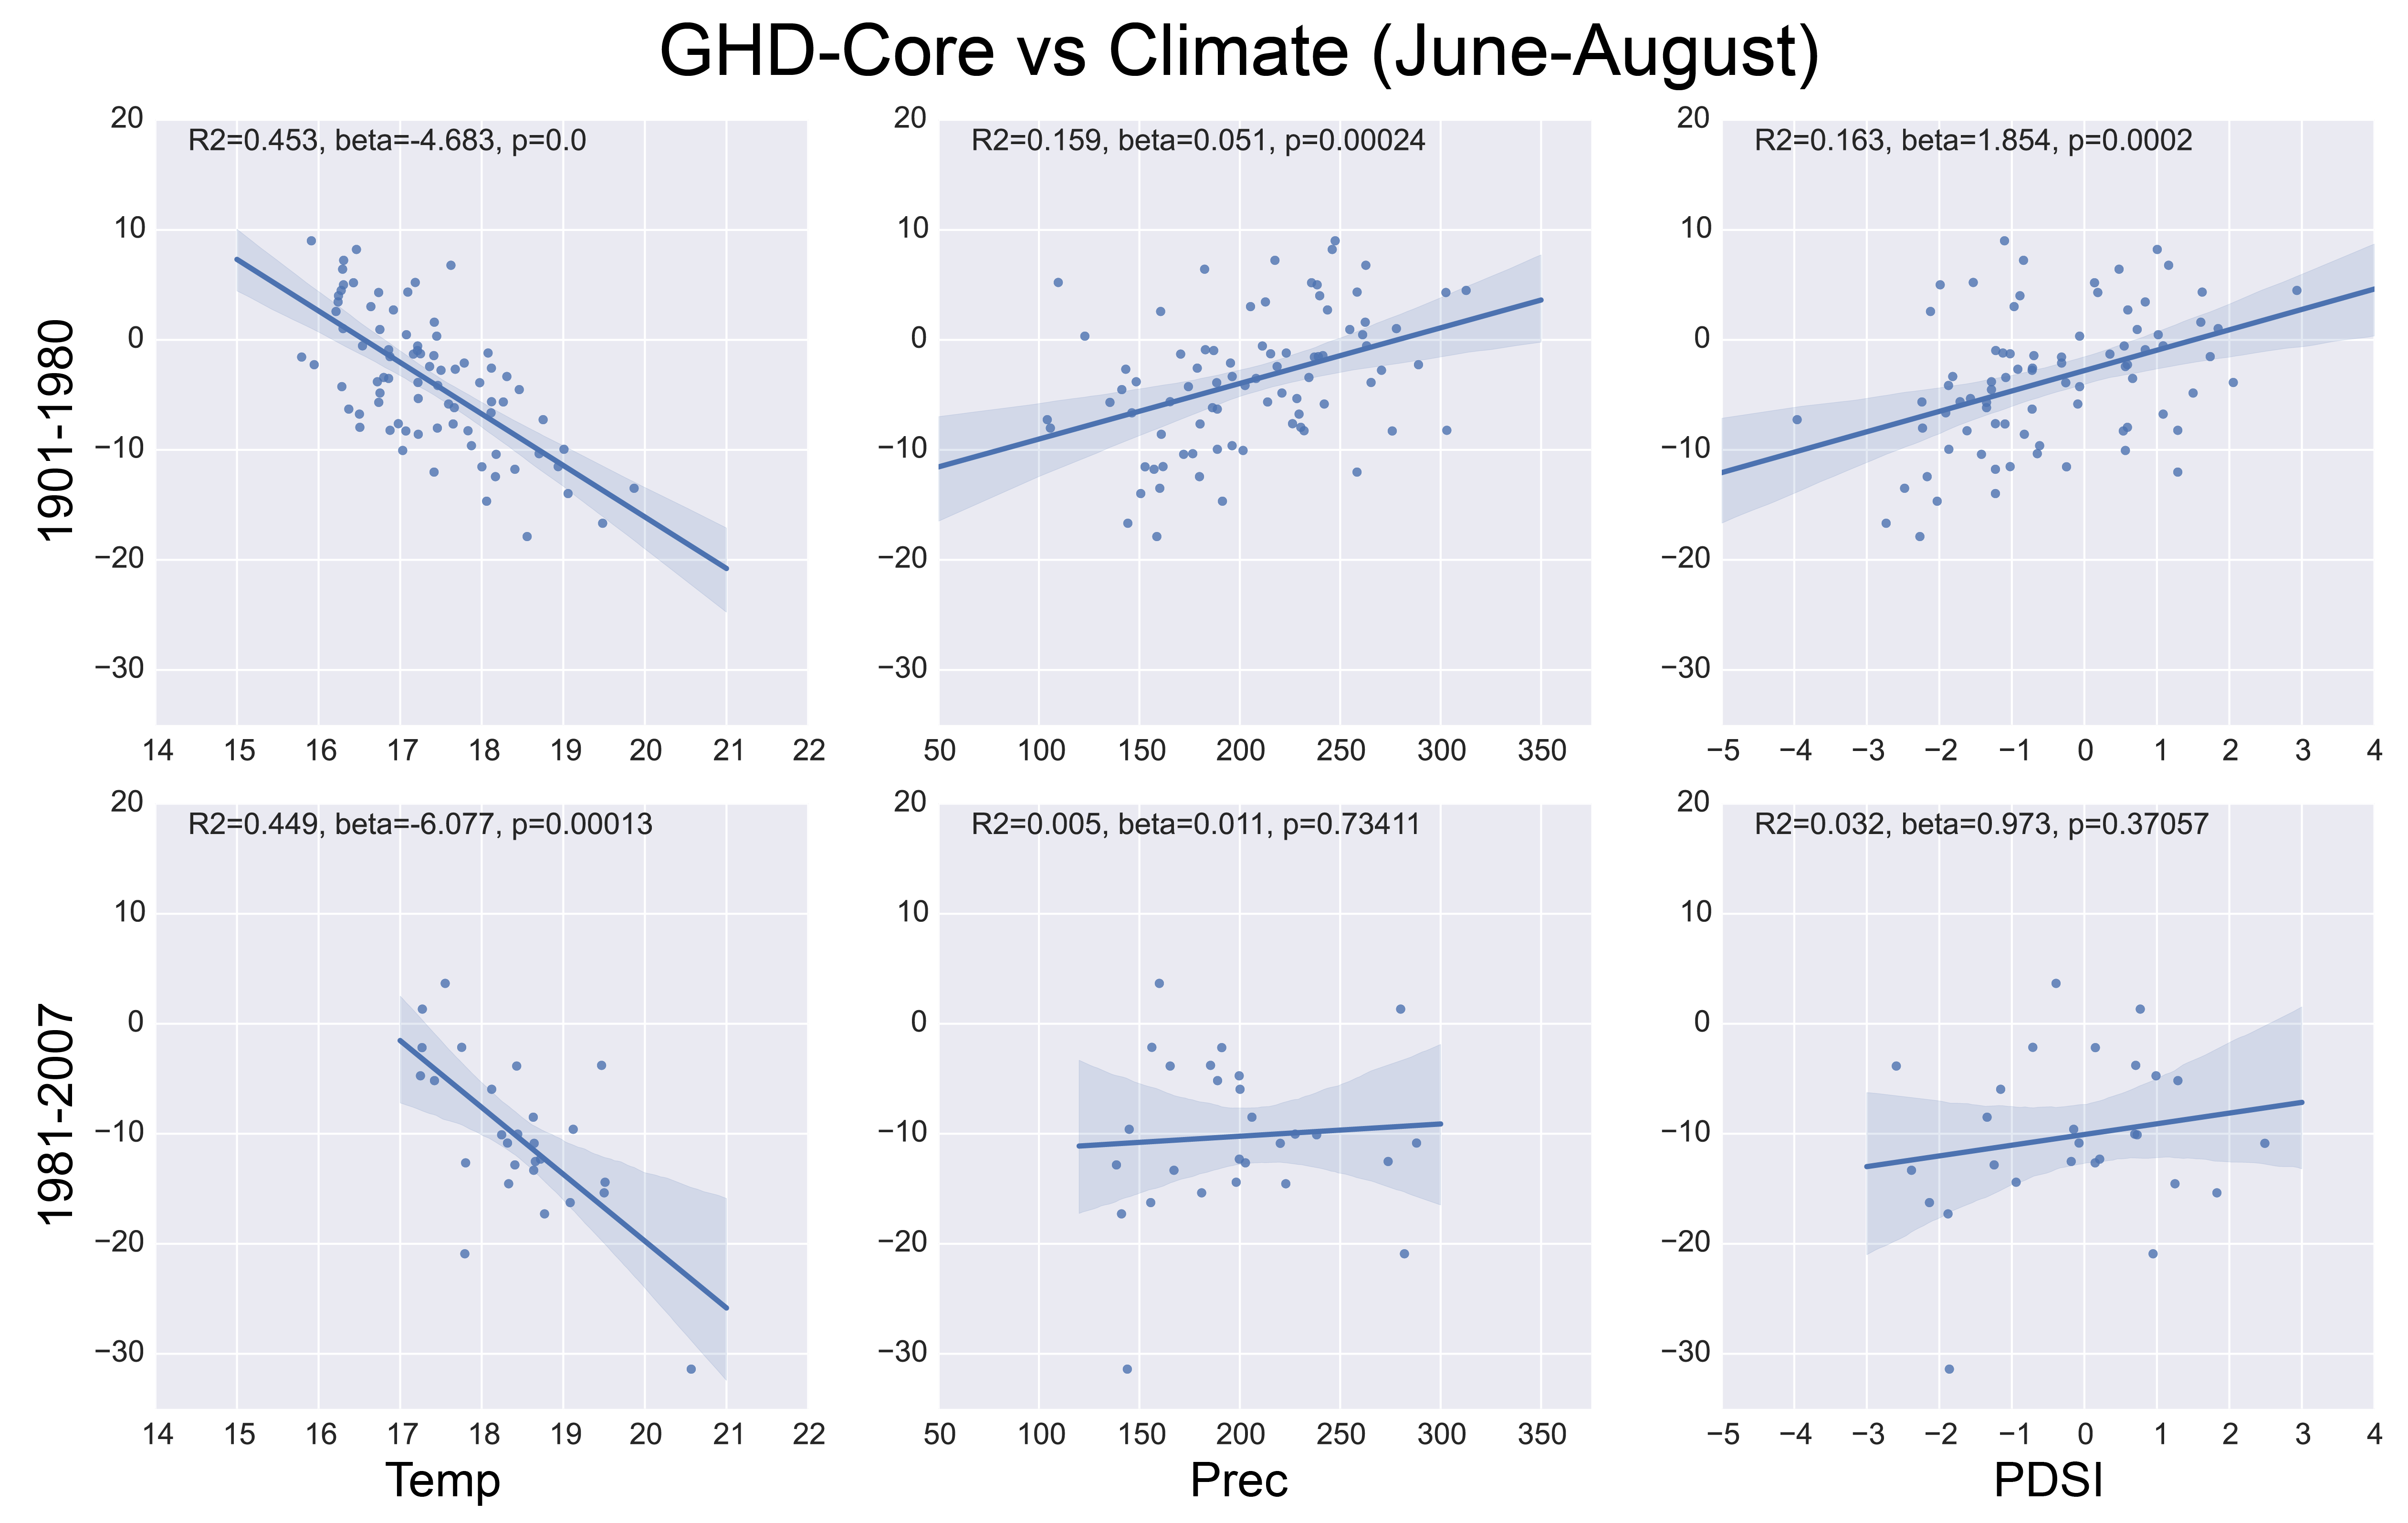
\includegraphics[width=1.0\columnwidth,scale=2]{SUPP_fig_13_JJA_clim_regplots.png}
\caption{Same as Figure 3 from the main manuscript, but for June-July-August (JJA).}
\end{figure}

\begin{figure}
\center
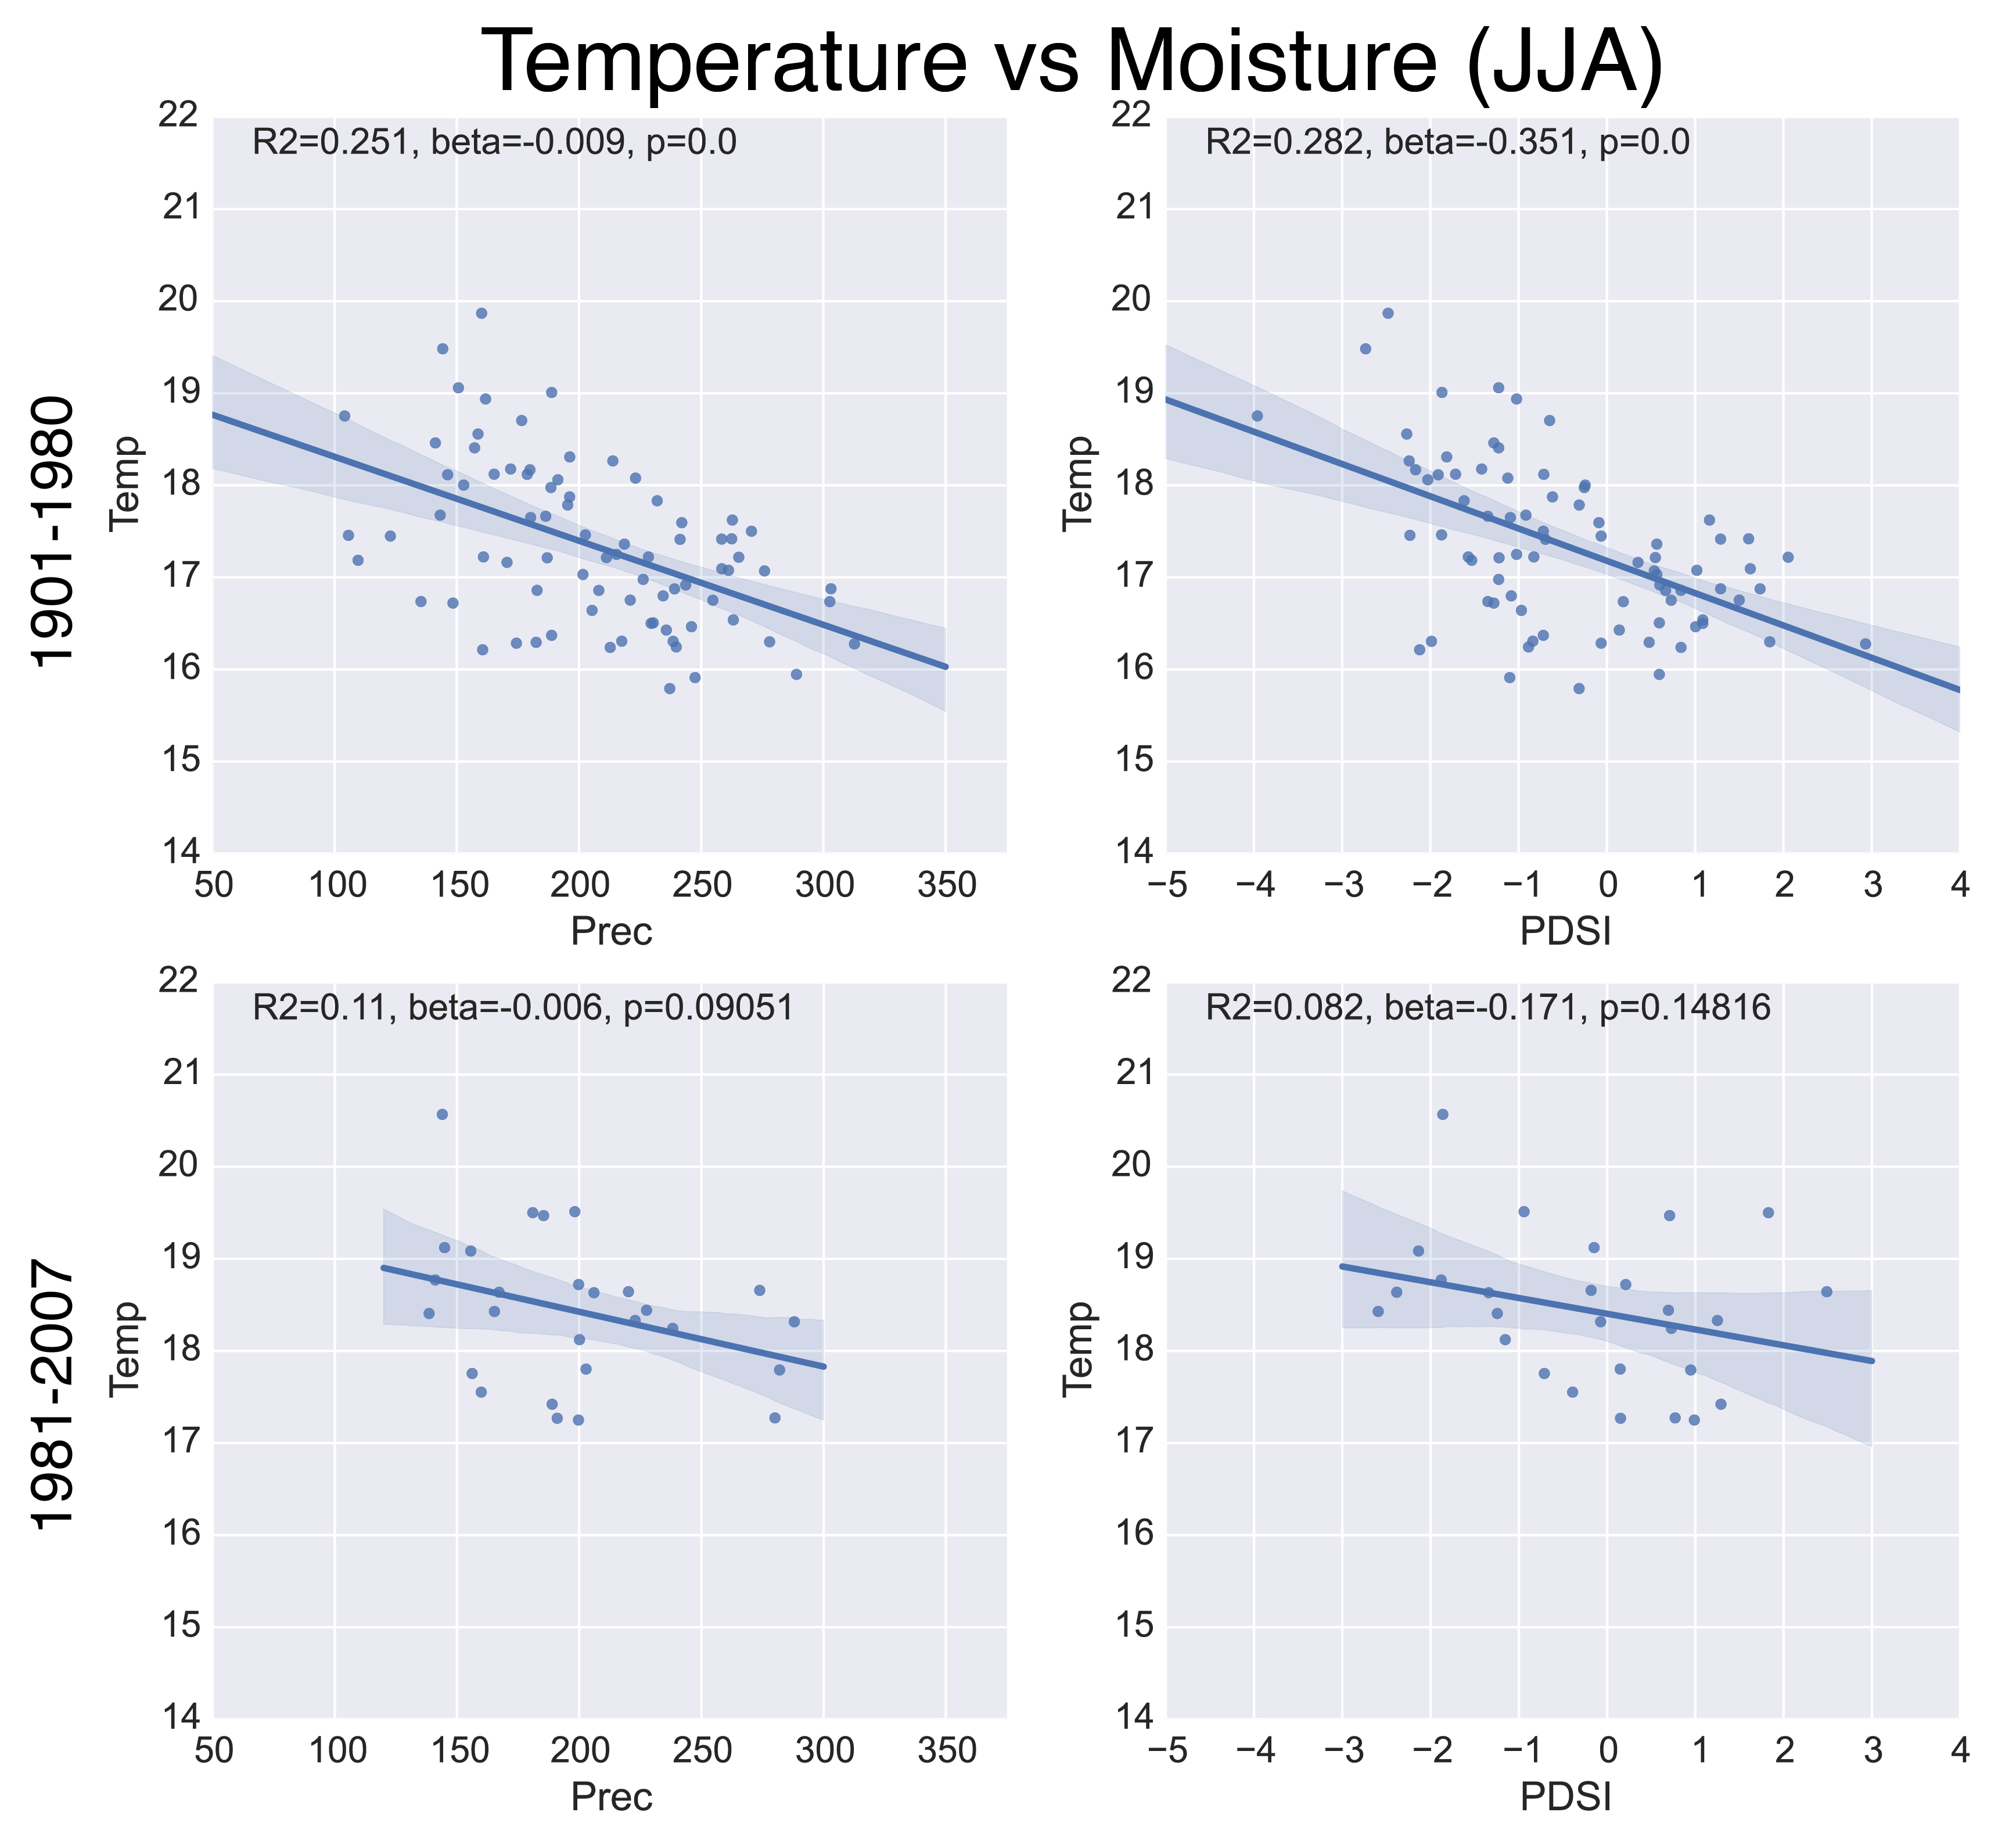
\includegraphics[width=1.0\columnwidth,scale=2]{SUPP_fig_14_temp_vs_moist_JJA.png}
\caption{Same as Supplemental Figure 11, but for June-July-August (JJA) climate. During JJA, the temperature moisture relationship is stronger over this region and, in both precipitation and PDSI, these relationships breakdown in the recent decades (1981--2007).}
\end{figure}

\begin{figure}
\center
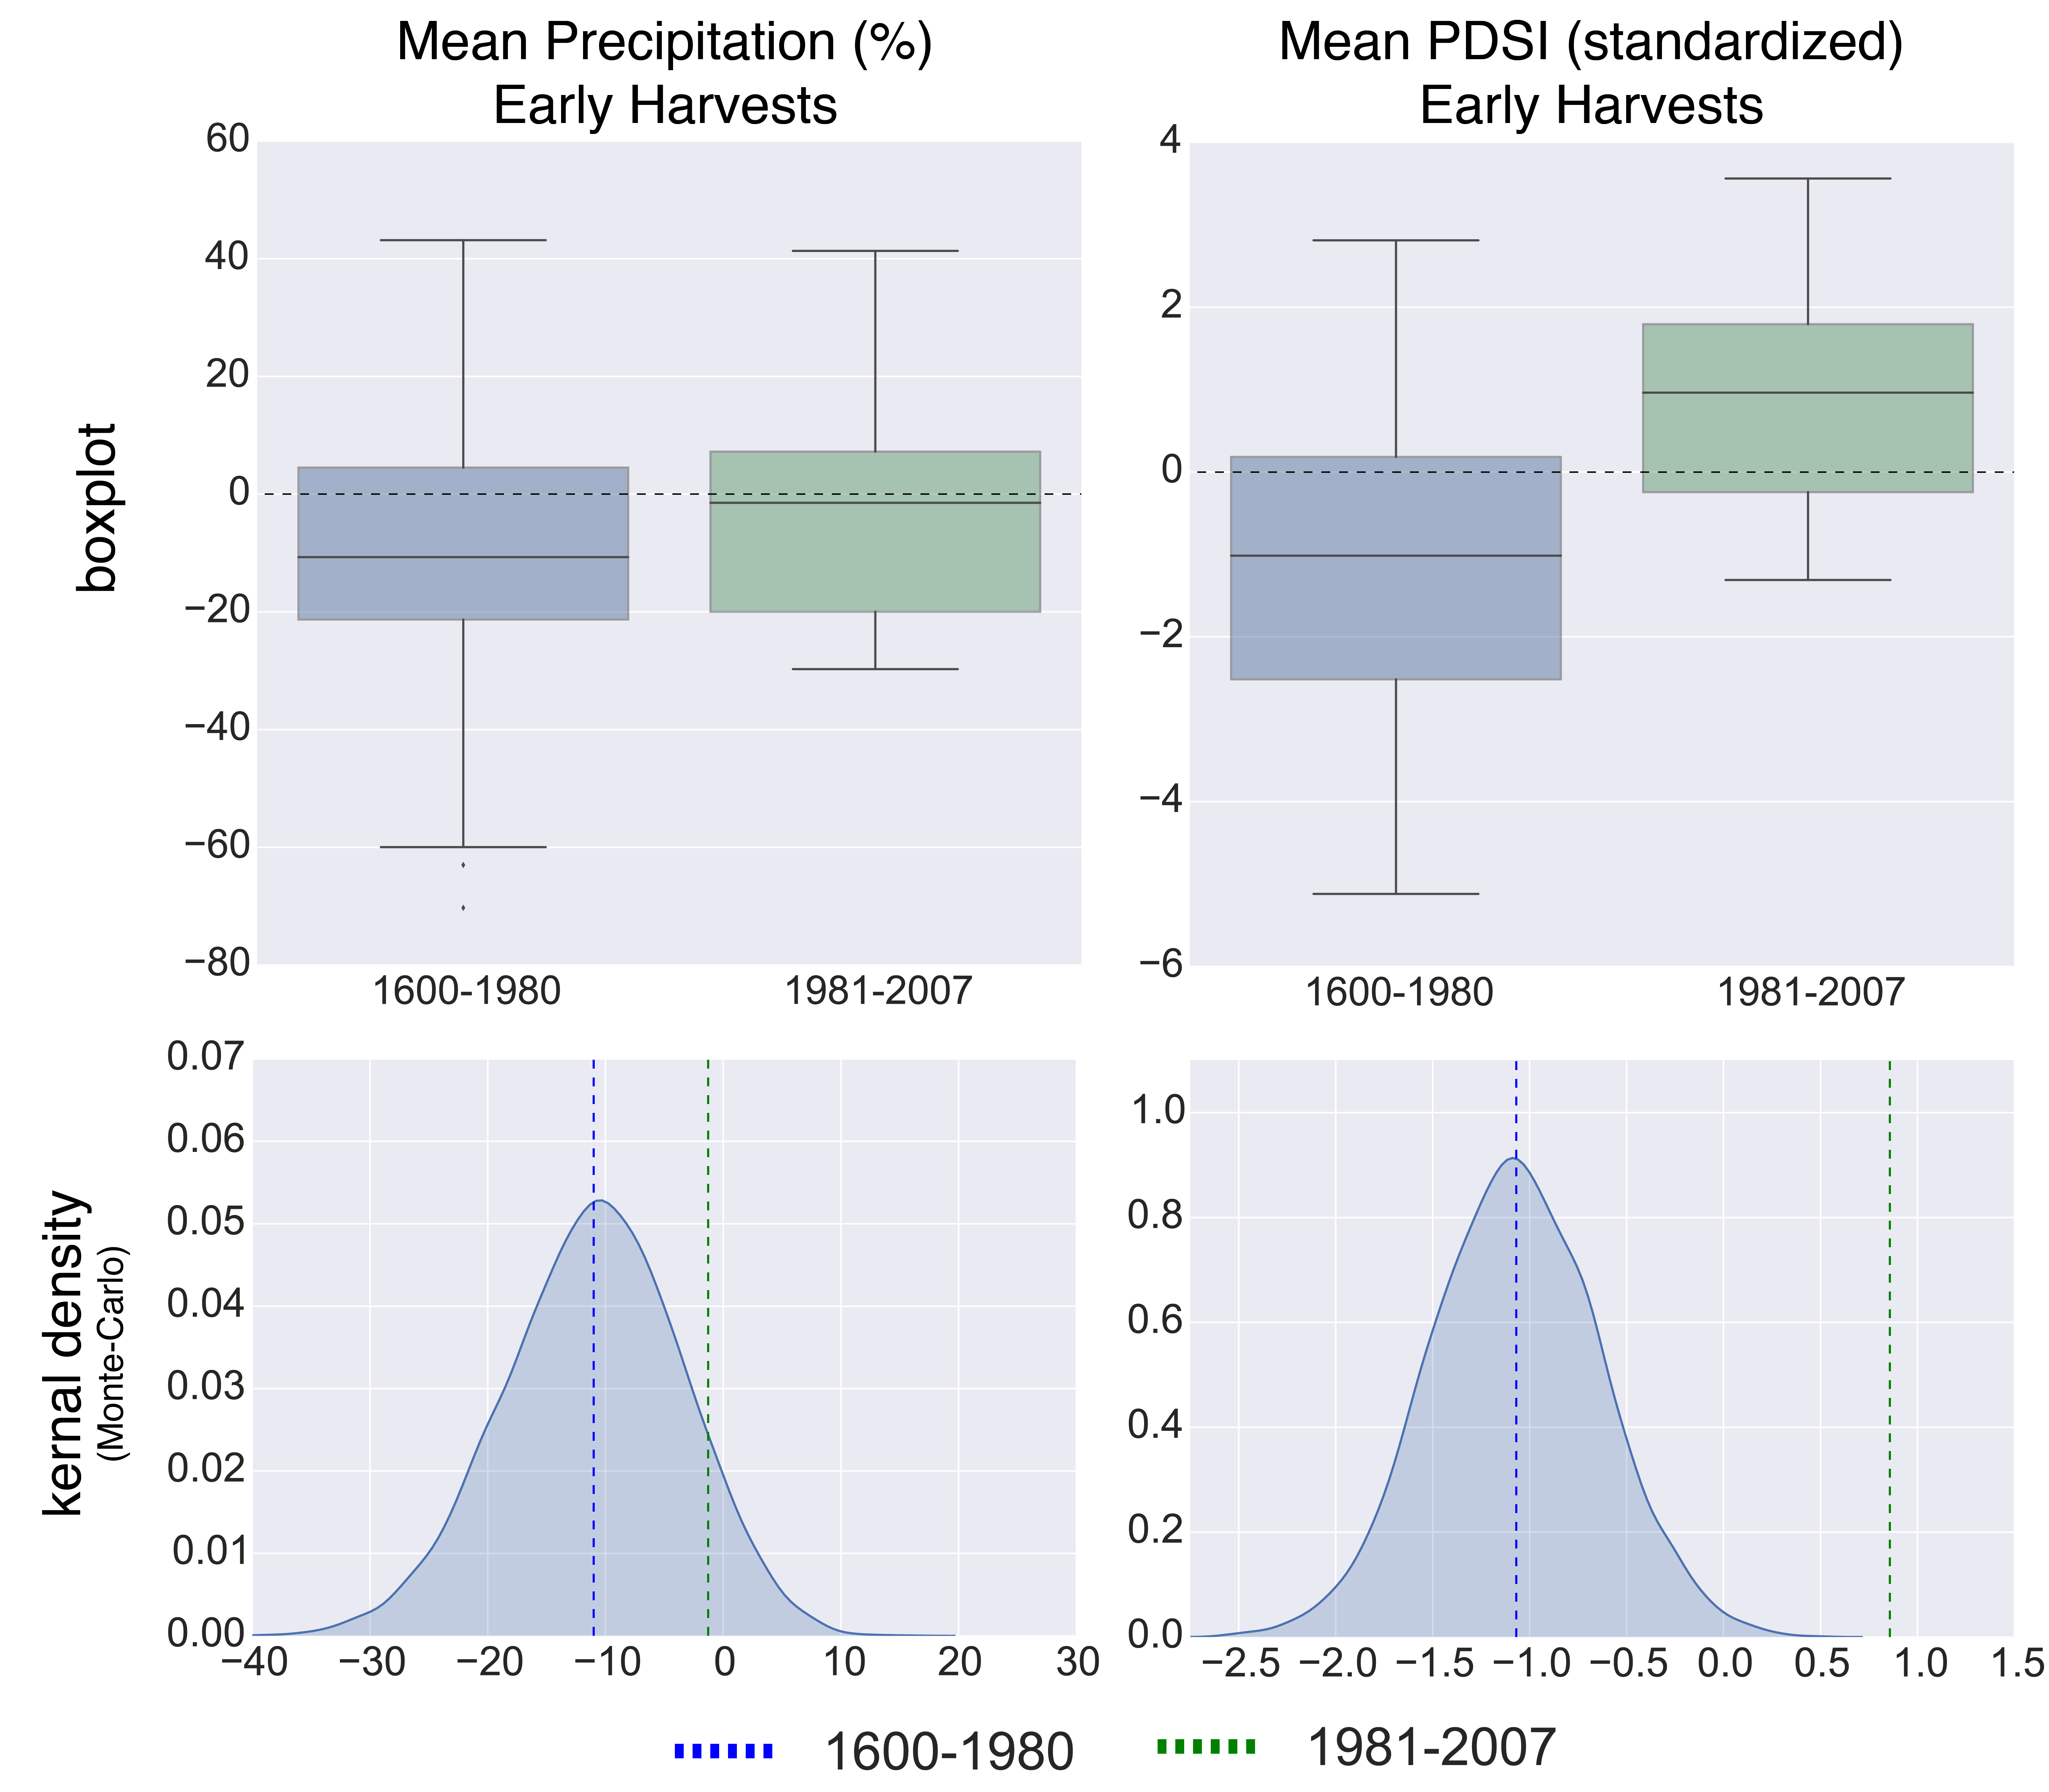
\includegraphics[width=1.0\columnwidth,scale=2]{SUPP_fig_15_JJA_boxplot_monte.png}
\caption{Top row: box plots of pooled precipitation and PDSI anomalies from the climate reconstructions for years with early harvest date anomalies in GHD-Core. Bottom row: kernel density functions of recalculated mean precipitation and PDSI anomalies associated with early harvest dates, based on 10,000 Monte-Carlo resamplings with replacement.}
\end{figure}

\end{document}









